\documentclass[11pt]{article}

\usepackage[a4paper,margin=1in]{geometry}
\usepackage{amsmath,amssymb,bm}
\usepackage{booktabs}
\usepackage{graphicx}
\usepackage{array}
\usepackage{microtype}
\usepackage{natbib}
\usepackage{xcolor}
\usepackage[hidelinks]{hyperref}
\hypersetup{
  pdftitle={Seed-mass dependence of baryon-assisted black-hole growth in self-interacting dark matter haloes},
  pdfauthor={Dong-Biao Kang},
  pdfsubject={Time-dependent SIDM accretion with baryonic assembly, cooling, feedback, and velocity-dependent transport},
  pdfkeywords={self-interacting dark matter, black-hole seeds, baryonic potential, Bondi accretion, gravothermal transport}
}

\graphicspath{{figures/}}
\setlength{\emergencystretch}{3em}
\newcommand{\msun}{\,\mathrm{M}_{\odot}}
\newcommand{\kms}{\,\mathrm{km\,s^{-1}}}
\newcommand{\pc}{\,\mathrm{pc}}
\newcommand{\dd}{\mathrm{d}}
\newcommand{\SIDM}{\mathrm{SIDM}}
\newcommand{\NFW}{\mathrm{NFW}}
\newcommand{\Bondi}{\mathrm{Bondi}}
\newcommand{\Edd}{\mathrm{Edd}}

\title{Seed-mass dependence of baryon-assisted black-hole growth in self-interacting dark matter haloes}
\author{%
  Dong-Biao Kang\\
  \small Zhejiang GuangSha Vocational and Technological University of China\\
  \small Institute of Theoretical Physics, Chinese Academy of Sciences\\
  \small \texttt{dbkang@zjgsdx.edu.cn}
}
\date{}

\begin{document}
\maketitle

\begin{abstract}
We present a controlled numerical study of time-dependent black-hole growth in self-interacting dark matter (SIDM) haloes with an assembled baryonic potential.  The calculation extends a conducting-fluid treatment with a monotonicity-preserving reconstruction and Roe fluxes to a finite Hernquist gas reservoir, Eddington-limited baryonic accretion, evolving Bondi ambient conditions, radiative cooling, and a conservative subgrid capture prescription for small seeds.  A constant-cross-section validation suite reproduces the reference singular-isothermal-sphere and Navarro--Frenk--White growth histories: a $100\msun$ seed reaches $129\msun$ and $9.65\times10^{3}\msun$, respectively, after $2\,{\rm Myr}$ when conduction is active.  In the fiducial physical-cooling model, a $10^{5}\msun$ seed in a $10^{9}\msun$ halo at $z=30$ crosses $10^{7}\msun$ in $1.52$--$1.76\,{\rm Myr}$ across the two smallest completed inner boundaries, although its terminal mass remains $7.1\%$ boundary sensitive.  The nominal mass gain is $98.81\%$ SIDM supplied.  The baryonic response is non-monotonic in compactness, with a maximum at $a_b/r_s=0.02$ rather than at the smallest tested radius.  Physical cooling removes stored thermal feedback; under the adopted irreversible expansion model, mixed feedback expands the Hernquist radius by about a factor of two, dilutes the gas, and reduces dark accretion by $33\%$.  A conservative capture prescription shows that $10^2$--$10^4\msun$ seeds do not enter the rapid-growth branch in $2\,{\rm Myr}$.  The transition at a few $10^4\msun$ is bracketed, rather than uniquely located, because it depends on the capture coefficient and feeding boundary.  A Rutherford/Born velocity-dependent cross section removes the threshold crossing throughout the tested domain at low transition speed and retains only a small boundary-robust subset in the high-transport model.  The robust numerical result is strong seed-mass and transport dependence in the explored parameter domain, not a population-level prediction or a generic route from stellar remnants to $10^{7}\msun$.
\end{abstract}

\section{Introduction}

The existence of massive black holes at high redshift motivates growth channels that do not rely exclusively on long episodes of ordinary baryonic Eddington accretion \citep{HaehneltRees1993,Salpeter1964,ShakuraSunyaev1973,BrommLoeb2003,MadauRees2001,Begelman2006,Volonteri2010,Inayoshi2020}.  Self-interacting dark matter provides a complementary possibility.  Elastic scattering can conduct heat through a halo, alter the central phase-space structure, and in the gravothermal regime drive a dense core toward collapse \citep{LyndenBellWood1968,SpergelSteinhardt2000,Balberg2002,KodaShapiro2011,Kaplinghat2016,TulinYu2018}.  The same transport can couple a black hole to a large reservoir of dark matter without invoking gas cooling at the capture radius.  Recent work has connected SIDM core collapse to early massive-black-hole seeds and to the population of little red dots (LRDs) \citep{Feng2021,Feng2025,Jiang2026}.

\citet{Meng2026} solved the spherical conducting-fluid problem for a black hole embedded in singular-isothermal-sphere (SIS) and NFW initial profiles.  That calculation established an important numerical and physical baseline: conduction can suppress the late central density and accretion rate, while an SIS profile can still provide rapid growth from a $100\msun$ seed.  It does not, however, answer four questions that determine whether the mechanism is useful as a controlled growth model.  First, how does a baryonic potential assembled on a finite time scale modify the supply region?  Second, can a finite gas reservoir and feedback alter both the Bondi limiter and the dark-matter potential?  Third, is the apparent runaway present for stellar-remnant seeds, or does it require an already intermediate-mass seed?  Fourth, does the conclusion survive a velocity-dependent SIDM cross section and a controlled scan in halo and baryonic parameters?

Here we answer these questions with a sequence of matched experiments.  The simulations remain one-dimensional and spherical, so the goal is not a cosmological population model.  Instead, we test the local model and identify which statements survive numerical, boundary, and microphysical checks.  We use a finite-volume MC reconstruction, Roe approximate Riemann flux, Harten entropy correction, and an implicit conduction update.  The baryons are represented by an evolving Hernquist reservoir \citep{Hernquist1990}; their assembly history is a smoothstep function, and feedback is split into thermal and expansion channels.  This extends earlier studies of baryonic potentials in gravothermal SIDM evolution \citep{Zhong2023} to a time-dependent accretion problem.  The gas state used by the Bondi rate is evolved with the reservoir and a no-ultraviolet-background Cloudy/Grackle cooling table \citep{Ferland2017,Smith2017}.  For small seeds, the resolved inward flux is separated from the unresolved capture rate by a mass-conserving central reservoir.

The paper has three deliberately distinct levels of claim.  The first is code validation against the reference SIS/NFW problem and a suite of grid, CFL, entropy-fix, and outer-boundary tests.  The second is a physical interpretation of the baryonic assembly and feedback response.  The third is an applicability map in which the scientific classifier is whether $10^7\msun$ is crossed within $2\,{\rm Myr}$; terminal masses are reported, but are not promoted to precision predictions when the inner boundary changes them by more than the pre-declared $5\%$ criterion.  We leave seed abundances, LRD number densities, and observables to a separate population study.

\section{Model}
\label{sec:model}

\subsection{Spherical SIDM fluid}

We evolve density $\rho$, radial velocity $u$, and one-dimensional velocity-dispersion variable $v$.  The pressure is $P=\rho v^2$.  In physical units the mass and momentum equations are
\begin{align}
 \frac{\partial \rho}{\partial t} + \frac{1}{r^2}\frac{\partial}{\partial r}(r^2\rho u) &= 0, \\
 \frac{\partial u}{\partial t}+u\frac{\partial u}{\partial r} &= -\frac{1}{\rho}\frac{\partial P}{\partial r} - \frac{G M_{\rm tot}(<r,t)}{r^2} .
\end{align}
The internal-energy equation is written in the form used by the conducting-fluid formulation,
\begin{equation}
 \frac{3}{2}\rho\frac{D v^2}{D t} = -P\frac{1}{r^2}\frac{\partial (r^2u)}{\partial r} - \frac{1}{r^2}\frac{\partial (r^2q_r)}{\partial r},
 \qquad q_r=-\kappa\frac{\partial v^2}{\partial r} .
 \label{eq:energy}
\end{equation}
The enclosed mass includes the black hole, dark matter, and the baryonic Hernquist component.  The transport closure is the usual harmonic interpolation between short- and long-mean-free-path limits,
\begin{equation}
 \kappa = \frac{3}{2}\left[\frac{\sigma/m}{Bv} + \frac{1}{A C\rho v^3(\sigma/m)}\right]^{-1},
 \qquad A=\sqrt{\frac{16}{\pi}},\quad B=\frac{25\sqrt{\pi}}{32},\quad C=\frac{3}{4} ,
 \label{eq:kappa}
\end{equation}
where $\sigma/m$ is the self-interaction cross section per unit mass.  This is an effective gravothermal fluid model rather than a collisionless particle calculation; its validity is therefore assessed against the baseline and against the expected transport limits \citep{Balberg2002,KodaShapiro2011,Outmezguine2023}.

The code uses dimensionless scales $M_0=4\pi\rho_0r_0^3$, $v_0=(GM_0/r_0)^{1/2}$, and $t_0=(4\pi G\rho_0)^{-1/2}$.  We retain physical units in tables and figures.  The reference initial halo is an NFW profile,
\begin{equation}
 \rho_{\NFW}(r)=\frac{\rho_s}{x(1+x)^2},\qquad x=r/r_s,
\end{equation}
with $M_{200}$, concentration $c=R_{200}/r_s$, and $M(<R_{200})=200(4\pi/3)\rho_{\rm crit}(z)R_{200}^3$ \citep{BryanNorman1998}.  SIS runs are used only as a validation control.  The NFW and SIS choices span the cored/contracting and centrally concentrated limits discussed in numerical SIDM studies \citep{Navarro1997,Dave2001,Rocha2013,Peter2013,Vogelsberger2012,Robertson2017}.

\subsection{Baryons and assembly}

The baryonic reservoir has a Hernquist enclosed mass
\begin{equation}
 M_b(<r,t)=M_{b,\rm rem}(t)\frac{r^2}{[r+a_b(t)]^2},
 \qquad \Phi_b(r,t)=-\frac{G M_{b,\rm rem}(t)}{r+a_b(t)} .
\end{equation}
The parameter $f_b$ denotes the fraction of $M_{200}$ made available to the assembled central reservoir; it is a model input, not an assertion that every high-redshift halo retains this baryon fraction.  Assembly is prescribed by
\begin{align}
 S(t)=\begin{cases}3\tau^2-2\tau^3,&0<\tau=t/T_{\rm asm}<1,\\1,&t\ge T_{\rm asm},\end{cases}
 \qquad M_{b,\rm asm}(t)&=f_bM_{200}S(t),\\
 M_{b,\rm rem}(t)&=\max\left[M_{b,\rm asm}(t)-\Delta M_{\rm gas}(t),0\right],
 \label{eq:assembly}
\end{align}
where $\Delta M_{\rm gas}$ is the cumulative gas mass removed by black-hole accretion, before the radiative-efficiency correction to the retained black-hole mass.  This smoothstep avoids an impulsive potential and permits a direct comparison between assembly time and local dynamical time.

The relevant local clocks are
\begin{equation}
 t_{\rm dyn}=\left[\frac{r^3}{G M_{\rm tot}(<r)}\right]^{1/2},\quad
 t_{\rm coll}=\left[a\rho(\sigma/m)v\right]^{-1},\quad
 t_{\rm cond}=\frac{3\rho L^2}{2\kappa},\quad
 t_{\rm in}=\frac{r}{|u|} .
 \label{eq:clocks}
\end{equation}
The supply radius is the logarithmic-radius median of the inward flux inside $r_s$.  Timescales are evaluated in the initial no-baryon hydrostatic state at that radius, so the correlation is a pre-run diagnostic rather than a circular fit to the evolved state.

\subsection{Gas accretion and feedback}

The black-hole mass is separated into dark and baryonic channels,
\begin{equation}
 \dot M_{\rm BH}=\dot M_{\rm DM}+\dot M_{b,{\rm BH}} .
\end{equation}
The gas supply is limited by the minimum of the Bondi and Eddington rates \citep{Bondi1952},
\begin{align}
 \dot M_{\Bondi} &=4\pi\lambda_B\frac{G^2M_{\rm BH}^2\rho_{\infty}(t)}{[c_s^2(t)+v_{\rm rel}^2]^{3/2}}, \\
 \dot M_{\Edd}&=\frac{4\pi G M_{\rm BH}m_p}{\epsilon_r\sigma_T c},\qquad
 \dot M_{b,{\rm BH}}=(1-\epsilon_r)\min(\dot M_{\Bondi},\dot M_{\Edd}) .
 \label{eq:bondi}
\end{align}
We use the standard adiabatic Bondi coefficient $\lambda_B=1/4$ for $\gamma=5/3$, $\epsilon_r=0.1$, and zero relative velocity in the one-zone gas model.  The Eddington cap applies only to the baryonic term in equation~(\ref{eq:bondi}); $\dot M_{\rm DM}$ is non-radiative in this model and is not Eddington limited.  The instantaneous total black-hole mass, including captured dark matter, nevertheless enters $\dot M_{\Edd}$ because it sets the gravitational mass relevant to the gas flow.  Dark accretion can therefore raise the subsequent baryonic Eddington ceiling without itself producing the associated radiation.

The ambient density and sound speed are coupled to the finite reservoir,
\begin{align}
 \rho_\infty(t)&=\rho_{\infty,0}\frac{M_{b,\rm rem}(t)}{M_{b,0}}\left[\frac{a_{b,0}}{a_b(t)}\right]^3,\\
 c_s^2(t)&=c_{s,0}^2+\frac{\gamma(\gamma-1)E_{\rm th}(t)}{M_{b,\rm rem}(t)} .
 \label{eq:ambient}
\end{align}
The feedback energy is split into a thermal reservoir and an irreversible expansion channel,
\begin{align}
 \frac{\dd E_{\rm th}}{\dd t}&=\chi_{\rm heat}\epsilon_f\epsilon_r\dot M_{\rm gas}c^2-\frac{E_{\rm th}}{t_{\rm cool}},\\
 a_b(t)&=a_{b,0}\left[1+\frac{(1-\chi_{\rm heat})\epsilon_f\epsilon_r\Delta M_{\rm gas}c^2}{E_{\rm bind,eff}}\right]^\eta, \\
 E_{\rm bind,eff}&=\frac{G M_{b,0}^2}{6a_{b,0}}+|W_{b,{\rm NFW}}|+\frac{G M_{{\rm BH},0}M_{b,0}}{a_{b,0}} .
 \label{eq:feedback}
\end{align}
Here $W_{b,{\rm NFW}}$ is the initial baryon--halo interaction energy, evaluated by radial quadrature in the NFW potential.  Unless stated otherwise, the fiducial calculation uses $\epsilon_f=10^{-3}$, $\chi_{\rm heat}=0.5$, $\eta=0.5$, primordial metallicity, and the unscaled tabulated cooling rate.  The feedback energy changes the baryonic source term, but is not directly injected into the SIDM energy equation.  The thermal reservoir is evolved implicitly because the Cloudy cooling time is state dependent.  We use the tabulated optically thin equilibrium coefficient in the range $10\le T/{\rm K}\le10^9$ and $-10\le\log_{10}(n_H/{\rm cm}^{-3})\le4$; primordial and solar-pattern metal contributions are linearly combined in $Z/Z_\odot$ \citep{Ferland2017,Smith2017}.  Inputs outside either tabulated axis are clipped to the nearest table boundary rather than extrapolated.  The initial $n_H\simeq9.2\times10^3\,{\rm cm^{-3}}$ is close to the upper density boundary, so this prescription and the omission of molecular cooling are explicit limitations.  The $10\kms$ initial sound speed is a floor representing the unheated hydrostatic state; cooling removes feedback heat, not this baseline support.

\subsection{Velocity-dependent transport}

For the final applicability map we replace the constant cross section by the Born/Rutherford angular law
\begin{equation}
 \frac{\dd\sigma}{\dd\Omega}=\frac{\sigma_0}{4\pi}\left[1+\left(\frac{v_{\rm rel}}{w}\right)^2\sin^2\frac{\theta}{2}\right]^{-2} .
 \label{eq:rutherford}
\end{equation}
Here $\theta$ is the center-of-mass scattering angle and $\sigma_0$ is the total cross section in the $v_{\rm rel}\rightarrow0$ limit, since the angular integral of equation~(\ref{eq:rutherford}) then equals $\sigma_0$.
The viscosity-weighted thermal averages are computed independently for the long- and short-mean-free-path terms,
\begin{equation}
 K_p=\frac{\langle\sigma_{\rm visc}v_{\rm rel}^p\rangle}{\langle\sigma_{\rm visc}v_{\rm rel}^p\rangle_{w\rightarrow\infty}},\quad
 \kappa_{\rm SMFP}=\frac{3Bv}{2\sigma_0K_5},\quad
 \kappa_{\rm LMFP}=\frac{3AC\rho v^3\sigma_0K_3}{2},
 \label{eq:velclosure}
\end{equation}
followed by the same harmonic interpolation as equation~(\ref{eq:kappa}).  A logarithmic quadrature and a 4097-point lookup table resolve the low-speed tail.  The constant-cross-section limit is recovered to $2\times10^{-10}$ in the regression test.  This separate $K_3/K_5$ treatment follows the transport prescription of \citet{Outmezguine2023}; replacing it by a single cross section at the virial velocity would miss the radial evolution of the inner transport.

The fiducial constant-cross-section solution spans both transport limits.  Its inner-cell Knudsen number decreases from $2.62\times10^{-2}$ initially to $1.15\times10^{-3}$ at $2\,{\rm Myr}$, placing the resolved inner region in the short-mean-free-path regime, while the radial median changes from $2.19$ to $0.846$ and the outer halo remains long mean free path.  The harmonic interpolation is therefore active across the simulated domain rather than serving only as a formal limiting prescription.

\section{Numerical method and validation}
\label{sec:numerics}

The radial mesh is logarithmic, with fixed physical inner and outer boundaries in a matched comparison.  The hyperbolic step is a finite-volume update using MC slopes in primitive variables, Roe fluxes \citep{Roe1981}, and a Harten entropy correction \citep{Harten1983}.  The reconstruction is monotonicity preserving in each cell and falls back to a first-order state when a characteristic extrapolation would produce a non-positive density or pressure.  The conduction term is operator split and advanced with a frozen-coefficient implicit tridiagonal solve.  Gravity and accretion sources are integrated after the hydrodynamic flux update.  These choices follow standard high-resolution finite-volume practice \citep{VanLeer1977,Toro2009} while retaining the conduction update of the reference calculation.

The absorbing inner boundary supplies the dark-matter channel in the resolved heavy-seed runs.  Each accepted result records the mass-budget residual, defined as the difference between initial dark mass, evolved dark mass, and the integrated inner flux in code units.  Across the numerical-sensitivity and applicability calculations the largest residual is $1.96\times10^{-10}$; this is negligible compared with the boundary differences discussed below.

We use $5\%$ as a pre-declared \emph{operational} tolerance for terminal-mass sensitivity, not as a universal SIDM standard or a proof of asymptotic convergence.  For two calculations it is evaluated with the symmetric relative difference
\begin{equation}
 \delta(M_1,M_2)=\frac{2|M_1-M_2|}{|M_1|+|M_2|},
 \label{eq:tolerance}
\end{equation}
and a terminal mass passes only when both the selected grid and inner-boundary differences have $\delta<0.05$.  The value was fixed before classifying the parameter survey: it lies safely above the $0.05$--$1.1\%$ baseline grid changes, but below the $10$--$60\%$ boundary excursions that generate spurious high-mass branches.  A different convention, such as $3\%$ or $10\%$, would change some terminal-mass labels.  For this reason we also report the physically coarser threshold classifier---whether both completed boundaries cross $10^7\msun$---which does not rely on assigning high precision to the endpoint.  This classifier is established only over the completed boundary bracket and is not an extrapolation to $r_{\min}\rightarrow0$.

\subsection{SIS/NFW baseline}

Figure~\ref{fig:baseline} shows the complete $2\,{\rm Myr}$ validation.  With conduction active, a $100\msun$ seed reaches $129.08\msun$ in the NFW halo and $9646.8\msun$ in the SIS halo, consistent with the reference endpoints \citep{Meng2026}.  Turning conduction off raises the endpoints to $234.36\msun$ and $32528.3\msun$, factors of $1.82$ and $3.37$, while the final inner densities increase by factors of $25.7$ and $104$.  This is the basic transport effect carried through the rest of the paper: conduction removes compressional heat from the inflowing region, but it also limits the central density available to the black hole.

\begin{figure}[t]
 \centering
 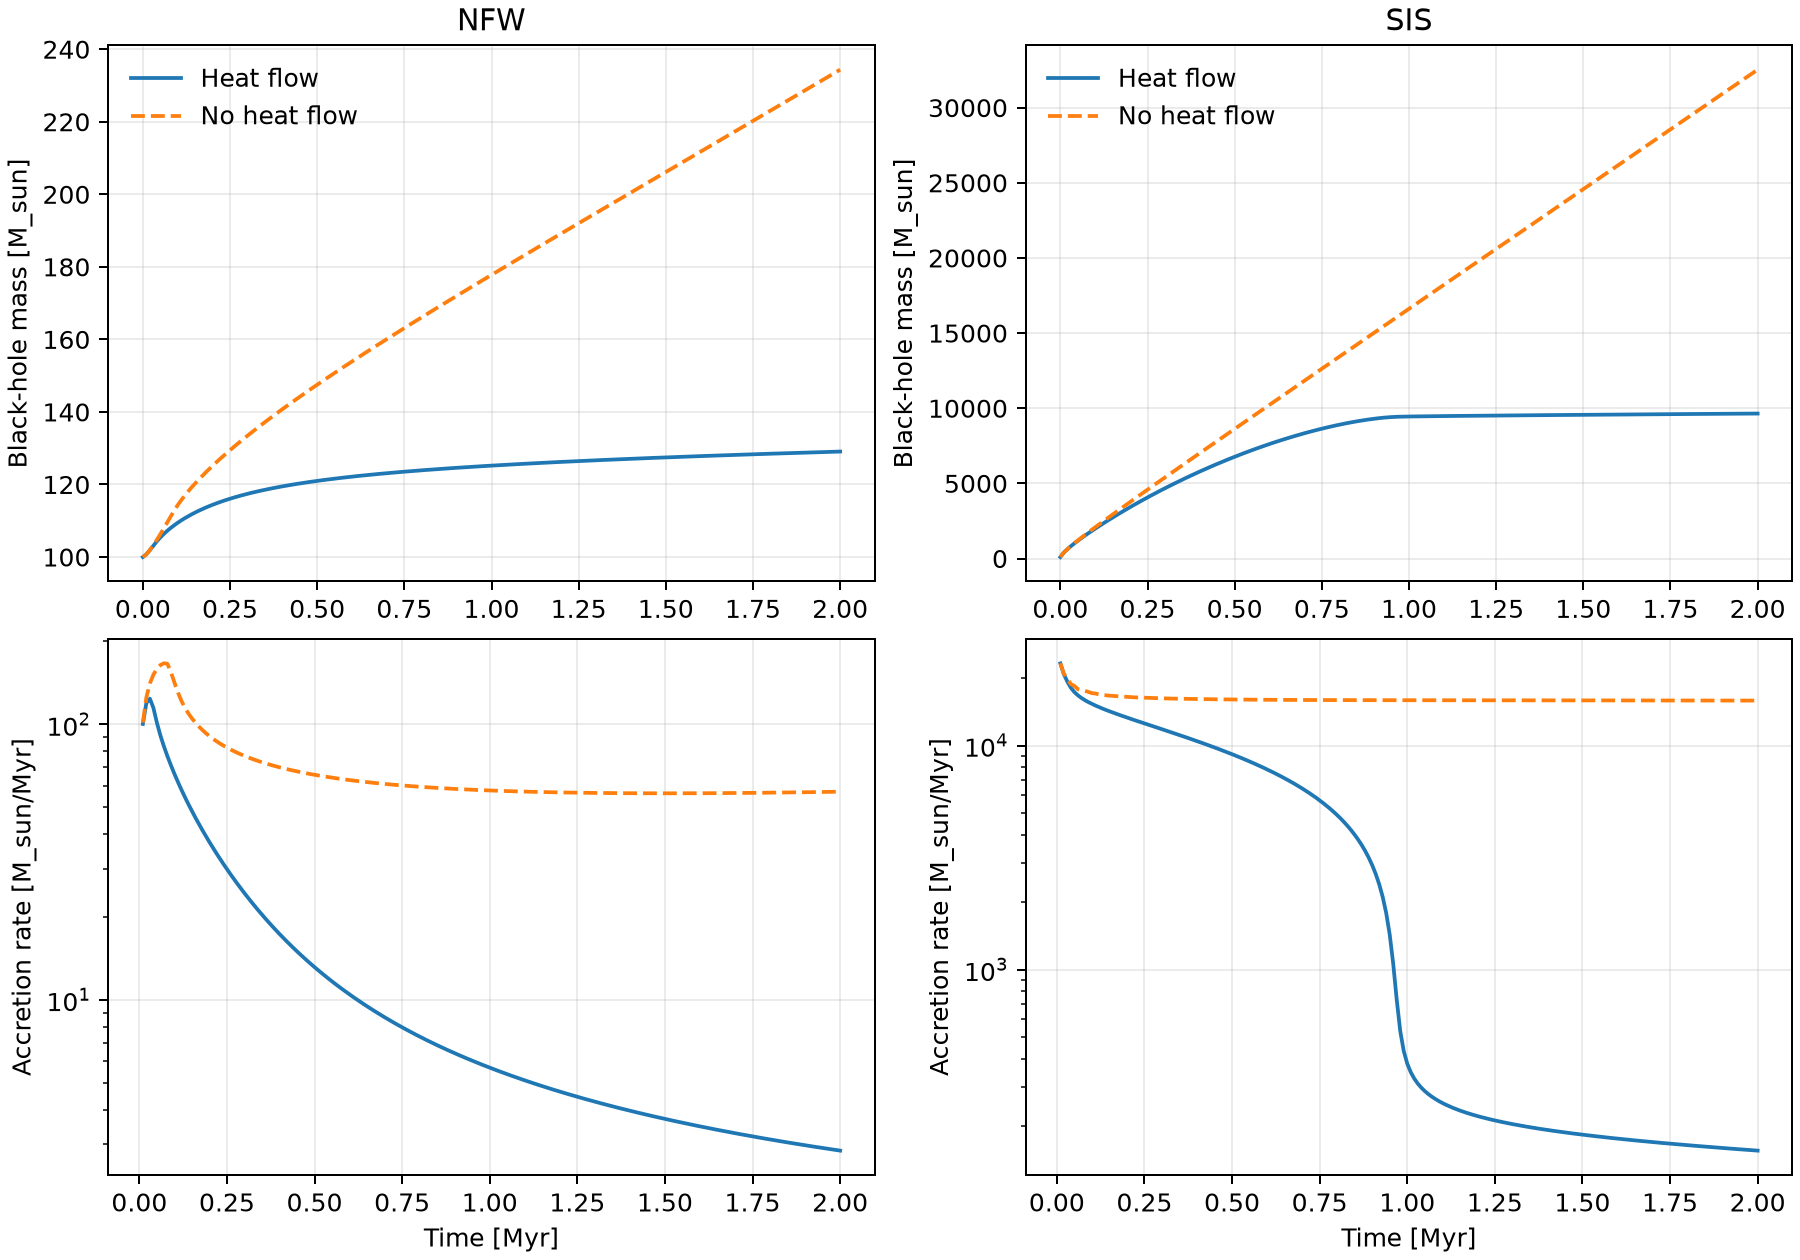
\includegraphics[width=0.98\linewidth]{baseline_growth_comparison.png}
 \caption{Baseline mass and accretion histories for NFW and SIS initial profiles.  The heat-on curves reproduce the reference $2\,{\rm Myr}$ endpoints, while heat-off curves show the large increase obtained when conductive transport is removed.}
 \label{fig:baseline}
\end{figure}

Grid, CFL, and entropy-fix tests are substantially smaller than the dominant inner-boundary systematic.  The NFW 256-to-512-cell change is $0.05\%$, the SIS change is $1.1\%$, CFL variations are below $0.012\%$, and varying the entropy-fix parameter changes the endpoint by less than $0.02\%$.  Changing the outer boundary over factors of four gives relative spans of $1.7\times10^{-6}$ (NFW) and $1.4\times10^{-4}$ (SIS).  In contrast, a factor-of-two inner-boundary shift changes the NFW endpoint by about $4\%$ and is larger in the more centrally concentrated SIS case.  We therefore retain at least two physical inner boundaries whenever a baryonic enhancement or threshold is quoted.

\section{Assembled baryonic potentials}
\label{sec:assembly}

\subsection{Mechanism and assembly clock}

The static Hernquist comparison is not sufficient: a pre-existing compact potential changes the initial hydrostatic support, whereas an assembled potential drives a transient response.  In the assembled experiments the dark-matter supply rises during baryon growth, reaches a broad maximum, and then declines.  Figure~\ref{fig:mechanism} compares the growth enhancement with the assembly time and with a heat-off control.  For $f_b=0.05$, $a_b/r_s=0.01$, and $\sigma/m=10$--$100\,\mathrm{cm^2\,g^{-1}}$, the refined optima are $T_{\rm asm}=0.50$--$0.75\,{\rm Myr}$.  The ratio $T_{\rm opt}/t_{\rm dyn}$ is $0.985$--$1.163$ with an RMS scatter of $0.046$ dex, whereas $T_{\rm opt}/t_{\rm coll}$ has a scatter of $0.545$ dex.  The particle collision time is therefore not the assembly clock.  A dynamical-time matching window is the more stable interpretation, in agreement with the idea that the potential must grow coherently with the region that supplies the black hole.

At the supply radius the $v^2$ gradient is negative in all refined conducting optima, so $q_r=-\kappa\partial_r v^2$ points outward.  The conductive term removes compressional heat from the inflowing region; it does not heat the center from outside.  When conduction is disabled the same finite-time optimum remains, but its enhancement is only $2.94$ rather than $26.7$--$102.4$.  The assembly window is therefore dynamical, while the large amplification is a transport effect.

\begin{figure}[t]
 \centering
 \begin{minipage}[t]{0.98\linewidth}
  \centering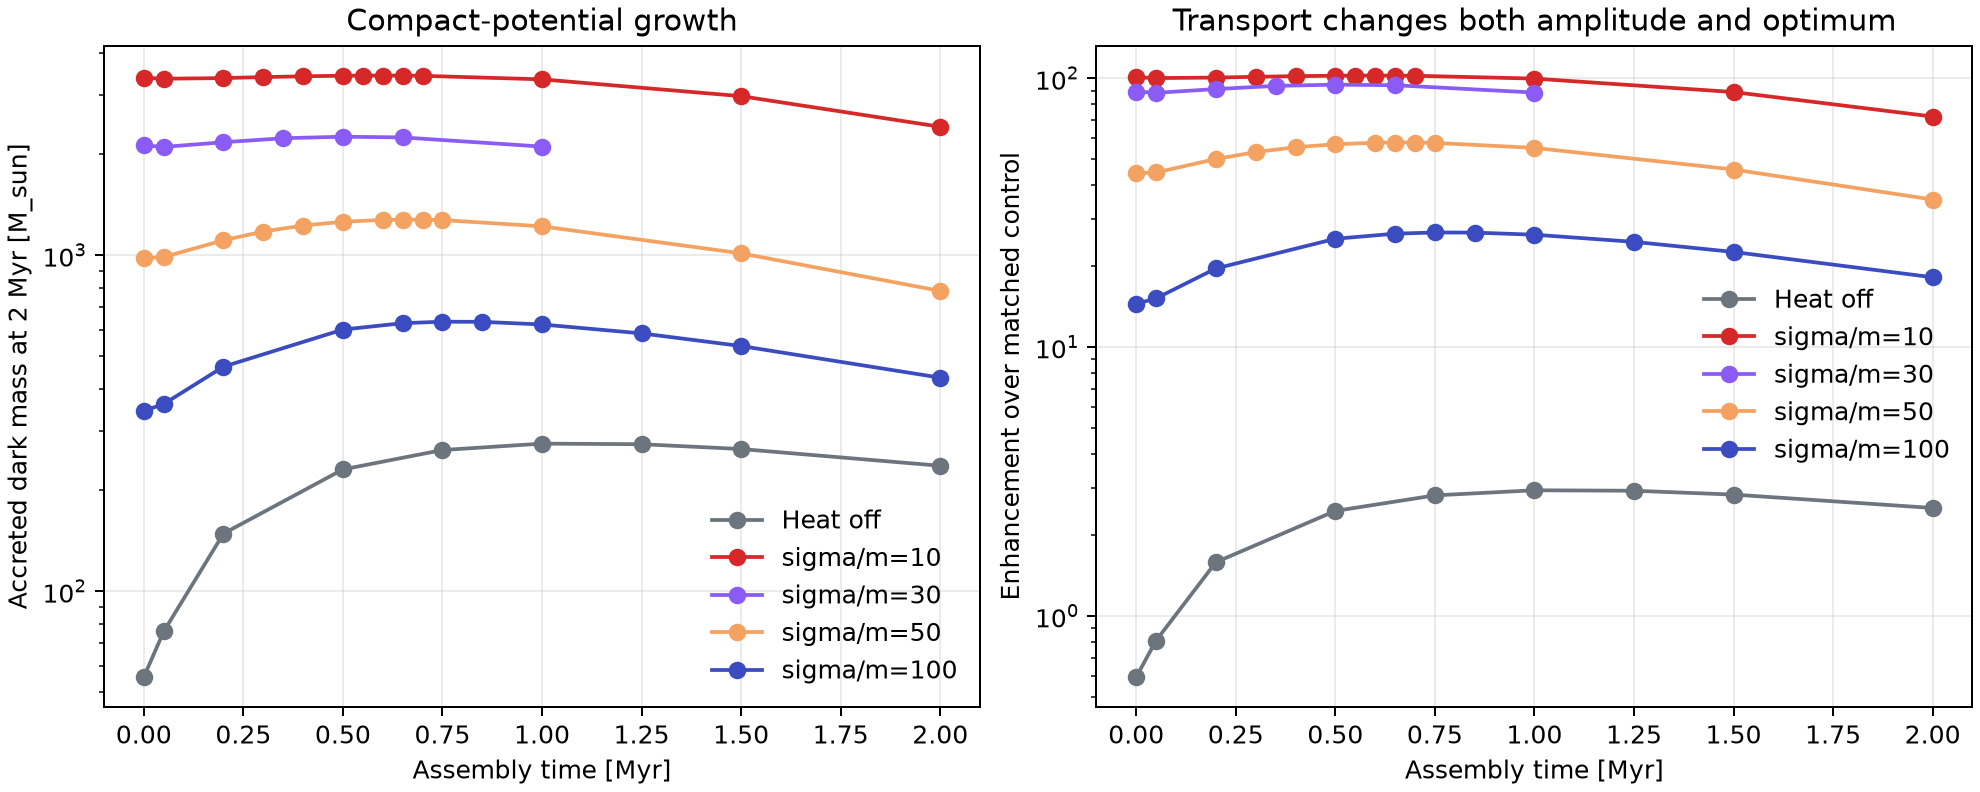
\includegraphics[width=\linewidth]{assembly_mechanism.png}
  \smallskip\centerline{(a) Compact-potential growth and transport enhancement.}
 \end{minipage}
 \\
 \begin{minipage}[t]{0.98\linewidth}
  \centering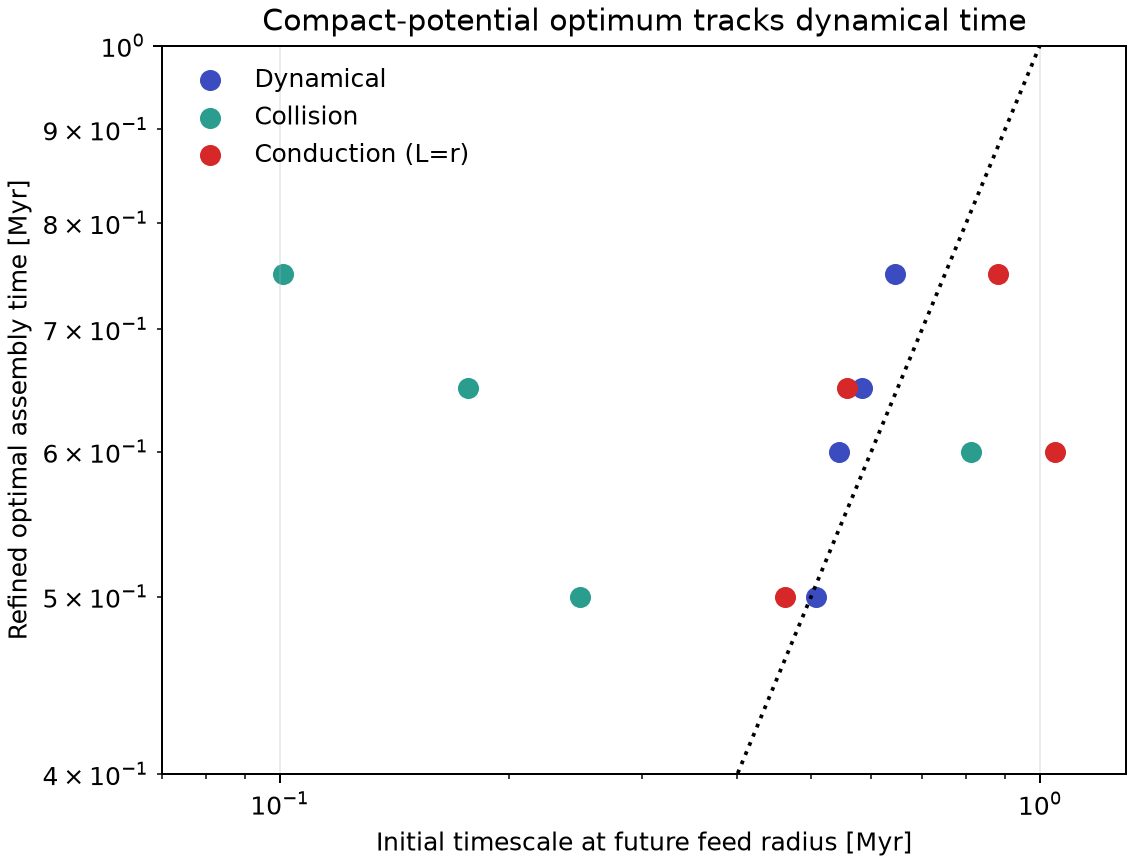
\includegraphics[width=\linewidth]{assembly_timescale_matching.png}
  \smallskip\centerline{(b) Refined assembly-time and initial-timescale comparison.}
 \end{minipage}
 \caption{The assembled baryonic potential creates a broad dynamical-time window rather than a narrow resonance.  Conductive transport sets the amplitude of the enhancement, and the heat-off curve is an adiabatic diagnostic rather than a collisionless model.}
 \label{fig:mechanism}
\end{figure}

\subsection{Compactness is non-monotonic}

The fiducial physical-cooling model adopts $M_{200}=10^9\msun$, $z=30$, $c=8$, $f_b=0.16$, $\sigma/m=1\,\mathrm{cm^2\,g^{-1}}$, and $T_{\rm asm}=1.25\,{\rm Myr}$.  The baryon fraction is an upper-reservoir assumption, and $c=8$ represents a deliberately high-concentration halo rather than a claim about the typical halo at $z=30$; the applicability calculations below span $c=4$--$12$.  The assembly-time interval $0.25$--$1.75\,{\rm Myr}$ was selected to bracket the local dynamical times of the resolved supply region, not as a cosmological distribution of assembly histories.  We rescan the baryonic scale radius at fixed physical boundaries.  The endpoint rises from $8.20\times10^6\msun$ at $a_b/r_s=0.003$ to $1.685\times10^7\msun$ at $a_b/r_s=0.020$, then falls to $1.473\times10^7\msun$ at $a_b/r_s=0.030$ (Table~\ref{tab:compactness}).  The most compact potential is not the best resolved case: its influence is deep but confined to too small a volume, and the smallest radii approach the inner boundary.  This is a physical scale-coupling result, not a claim that compactness is unimportant.

\begin{table}[t]
\centering
\caption{Compactness scan around the fiducial physical-cooling model.}
\label{tab:compactness}
\begin{tabular}{ccc}
\toprule
$a_b/r_s$ & $M_{\rm BH}(2\,{\rm Myr})/\msun$ & comment\\
\midrule
0.003 & $8.20\times10^6$ & resolved representative\\
0.005 & $1.12\times10^7$ & threshold crossing\\
0.0075 & $1.36\times10^7$ & threshold crossing\\
0.010 & $1.51\times10^7$ & threshold crossing\\
0.015 & $1.67\times10^7$ & near peak\\
0.020 & $1.685\times10^7$ & nominal peak\\
0.030 & $1.47\times10^7$ & post-peak\\
\bottomrule
\end{tabular}
\end{table}

\section{Evolving gas, cooling, and feedback}
\label{sec:feedback}

The gas problem contains a feedback loop: a larger black hole raises $\dot M_{\Edd}$, retained gas deepens the central potential, and feedback can expand that potential while modifying $\rho_\infty$ and $c_s$.  A no-feedback compact-halo baseline exhibits two-way catalysis, but remains dark dominated: in the earlier $10^6\msun$ test, full-Eddington runs from $10$--$1000\msun$ seeds have dark fractions of $96.9$--$99.0\%$.  This does not mean that baryons are dynamically irrelevant; it means that their role is to change the central environment rather than to provide most of the final mass in the short experiment.

The physically cooled calculation is more restrictive than a stored-heat model.  Under optically thin Cloudy cooling, pure heating at $\epsilon_f=10^{-3}$ retains only $0.033$--$0.159\%$ of the injected thermal energy and does not prevent the Bondi-to-Eddington transition.  Suppressing the cooling coefficient by $10^5$--$3\times10^5$ is required for heating alone to keep the gas Bondi limited.  This is a trapping requirement, not a small metallicity correction.  By contrast, under the adopted irreversible mixed-feedback model, assigning half of the feedback energy to expansion increases $a_b$ by about $1.9$ and decreases $\rho_\infty$ by a factor of $6.8$--$7.0$.  The gas then remains Bondi limited throughout $2\,{\rm Myr}$ and the dark channel is reduced by $32.8$--$33.1\%$ relative to the no-feedback control.  These percentages quantify sensitivity within this model; they are not a general prediction for resolved baryonic feedback.

\begin{figure}[t]
 \centering
 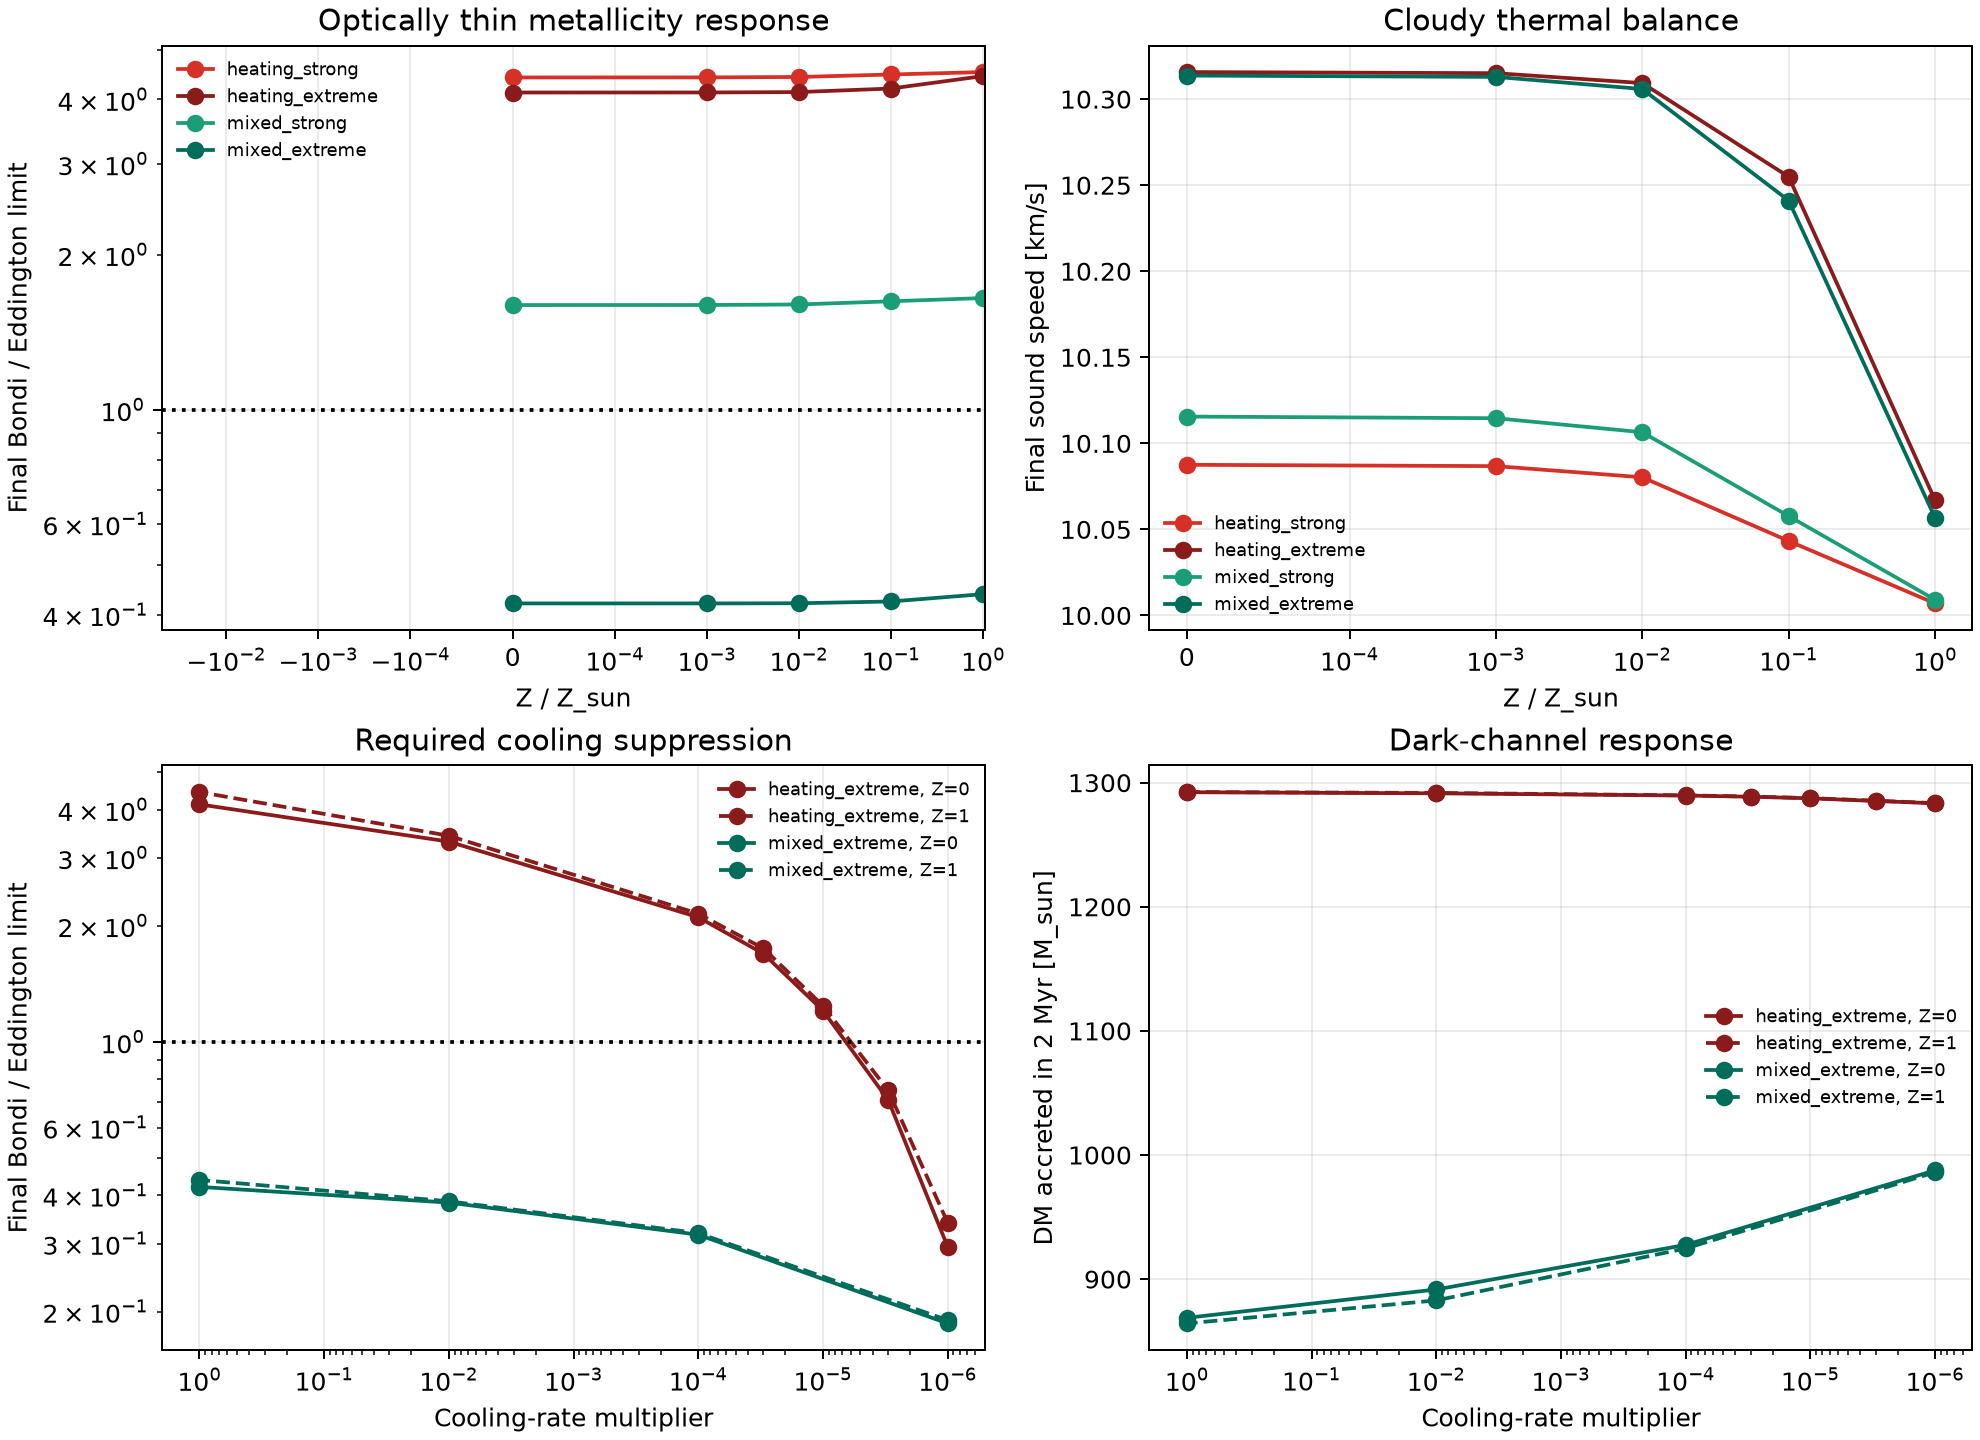
\includegraphics[width=0.98\linewidth]{physical_cooling_feedback.png}
 \caption{Physical cooling and feedback response.  The top panels show that metallicity has a secondary effect on the final limiter state and sound speed.  The lower panels show the large cooling suppression required by pure heating and the simultaneous dilution of the dark channel in the mixed expansion model.}
 \label{fig:cooling}
\end{figure}

The feedback threshold is therefore controlled by channel in the present model.  Heating is erased by cooling because $t_{\rm cool}$ is short, whereas homologous expansion is cumulative by construction.  Expansion can prevent the gas transition while suppressing the dark channel; it is not an independent mechanism that boosts both channels.  The sign of this response follows from weakening the central potential and diluting the gas, but its magnitude and persistence require a reversible radius equation or resolved gas dynamics.  The current prescription is irreversible, one-zone, and does not include an outflow or recontraction.

\section{Heavy-seed growth and numerical sensitivity}
\label{sec:heavyseed}

The best nominal model has $M_{\rm BH,0}=10^5\msun$.  At $a_b/r_s=0.02$ it reaches $1.6850\times10^7\msun$ at $2\,{\rm Myr}$, with $1.6551\times10^7\msun$ in dark accretion and $1.9883\times10^5\msun$ in retained baryons.  Thus $98.81\%$ of the total growth is dark.  The Hernquist radius expands from $2.507\pc$ to $2.615\pc$, the one-zone gas density falls from $0.300$ to $0.264\msun\,\pc^{-3}$, and the sound speed rises from $10.0$ to $11.99\kms$.

The endpoint is not fully converged under the strict $5\%$ terminal-mass criterion.  Doubling the grid from 256 to 512 cells changes the endpoint by only $0.298\%$, but reducing the physical inner boundary gives $1.5599\times10^7\msun$ and $1.4523\times10^7\msun$, a $7.14\%$ difference (Figure~\ref{fig:heavyseed}).  Every completed boundary variant crosses $10^7\msun$ at $1.52$--$1.76\,{\rm Myr}$, and the smallest endpoint remains $45.2\%$ above the threshold.  We therefore retain threshold crossing as a boundary-bracketed result, not as evidence of convergence under further unresolved boundary reduction, and label $1.685\times10^7\msun$ a nominal peak.

\begin{figure}[t]
 \centering
 \begin{minipage}[t]{0.98\linewidth}
  \centering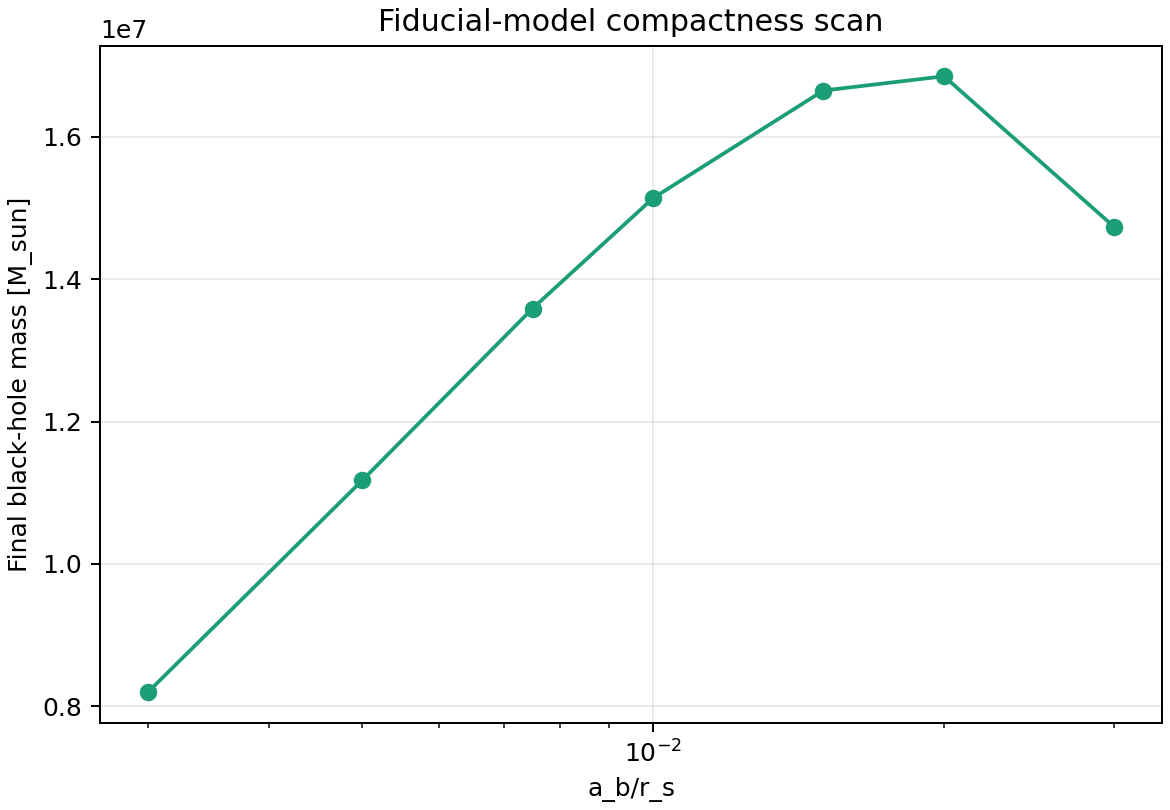
\includegraphics[width=\linewidth]{compactness_scan.png}
  \smallskip\centerline{(a) Resolved compactness peak.}
 \end{minipage}
 \\
 \begin{minipage}[t]{0.98\linewidth}
  \centering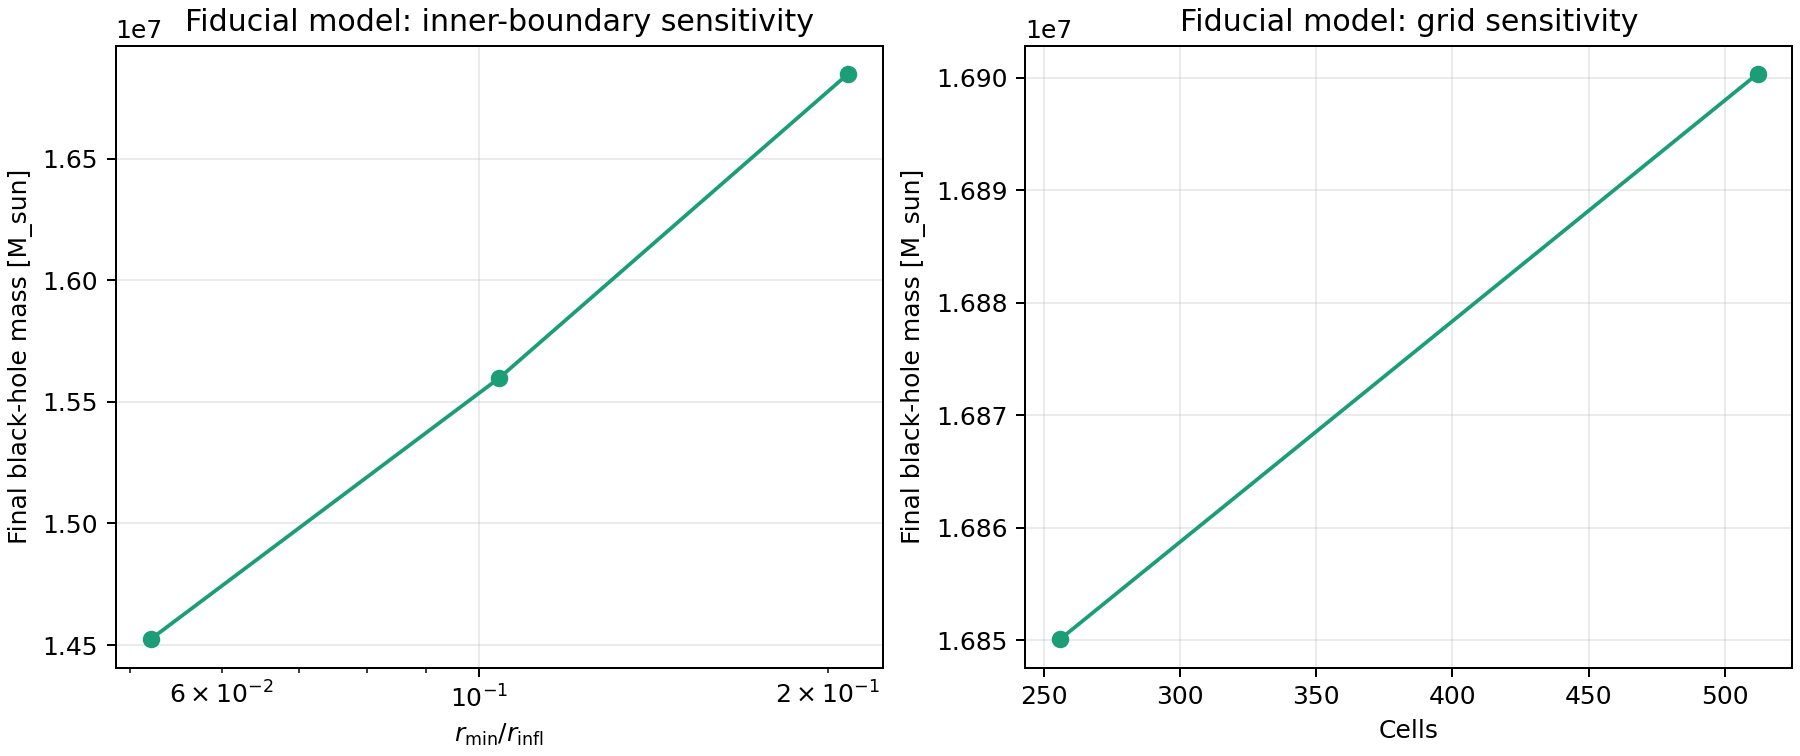
\includegraphics[width=\linewidth]{heavy_seed_numerical_sensitivity.png}
  \smallskip\centerline{(b) Grid and inner-boundary convergence.}
 \end{minipage}
 \caption{The preferred heavy-seed model has an internal compactness maximum, but the inner boundary remains the leading terminal-mass systematic.  The threshold crossing is more stable than the terminal mass.}
 \label{fig:heavyseed}
\end{figure}

\begin{table}[t]
\centering
\caption{Resolution and inner-boundary sensitivity of the fiducial $a_b/r_s=0.02$ model.}
\label{tab:convergence}
\begin{tabular}{lcc}
\toprule
variant & $M_{\rm BH}(2\,{\rm Myr})/\msun$ & $t(M_{\rm BH}=10^7\msun)$ [Myr]\\
\midrule
256 cells & $1.6850\times10^7$ & 1.53\\
512 cells & $1.6900\times10^7$ & 1.52\\
$r_{\min}/r_{\rm infl}=0.104$ & $1.5599\times10^7$ & 1.65\\
$r_{\min}/r_{\rm infl}=0.052$ & $1.4523\times10^7$ & 1.76\\
\bottomrule
\end{tabular}
\end{table}

The numerically unresolved high-mass branch is also informative.  Nominal $10^8\msun$-like endpoints occur at high concentration, high cross section, and extremely compact baryons, but their two smallest inner boundaries differ by $56$--$64\%$.  The apparent enhancement is an unresolved capture-boundary effect.  Grid, CFL, and entropy-fix changes are small in these cases; the failure is the unresolved absorbing-boundary treatment, not a hydrodynamic instability.

\section{Light seeds: delivery versus capture}
\label{sec:seeds}

Applying the heavy-seed absorbing flux directly to a $10^2\msun$ seed would make the physical inner boundary shrink by three orders of magnitude.  Instead we introduce a feeding radius and separate the resolved inward delivery from capture by the unresolved black hole,
\begin{align}
 \dot M_{\rm supply} &= \max[-4\pi r_{\rm feed}^2\rho(r_{\rm feed})u(r_{\rm feed}),0],\\
 \dot M_{\rm cap} &= 4\pi\lambda_B\frac{G^2M_{\rm BH}^2\rho(r_{\rm feed})}{c_s^3(r_{\rm feed})} .
 \label{eq:seedclosure}
\end{align}
Supplied but uncaptured dark matter enters a conservative central reservoir and contributes to the gravitational field.  Bondi capture operates while $r_{\rm feed}/r_{\rm infl}>0.104$; once the feeding radius is inside the influence region, the model switches to direct capture and drains the reservoir on a local free-fall time.  This capture prescription reproduces three directly resolved heavy-seed runs to $3.97\times10^{-6}$ in final mass and changes by only $2.42\times10^{-6}$ when the gate is moved across the tested bracket.

The fixed-halo seed ladder is summarized in Table~\ref{tab:seeds}.  A $10^2\msun$ seed supplies $1.42\times10^4\msun$ of dark matter to the feeding radius but captures only $3.25\msun$; a $10^3\msun$ seed captures $103\msun$ from $5.28\times10^4\msun$ supplied; and a $10^4\msun$ seed captures $7.17\times10^3\msun$ from $6.74\times10^6\msun$ supplied.  The capture fractions are $0.023\%$, $0.195\%$, and $0.106\%$.  Central delivery is therefore not equivalent to black-hole growth.

\begin{figure}[t]
 \centering
 \begin{minipage}[t]{0.98\linewidth}
  \centering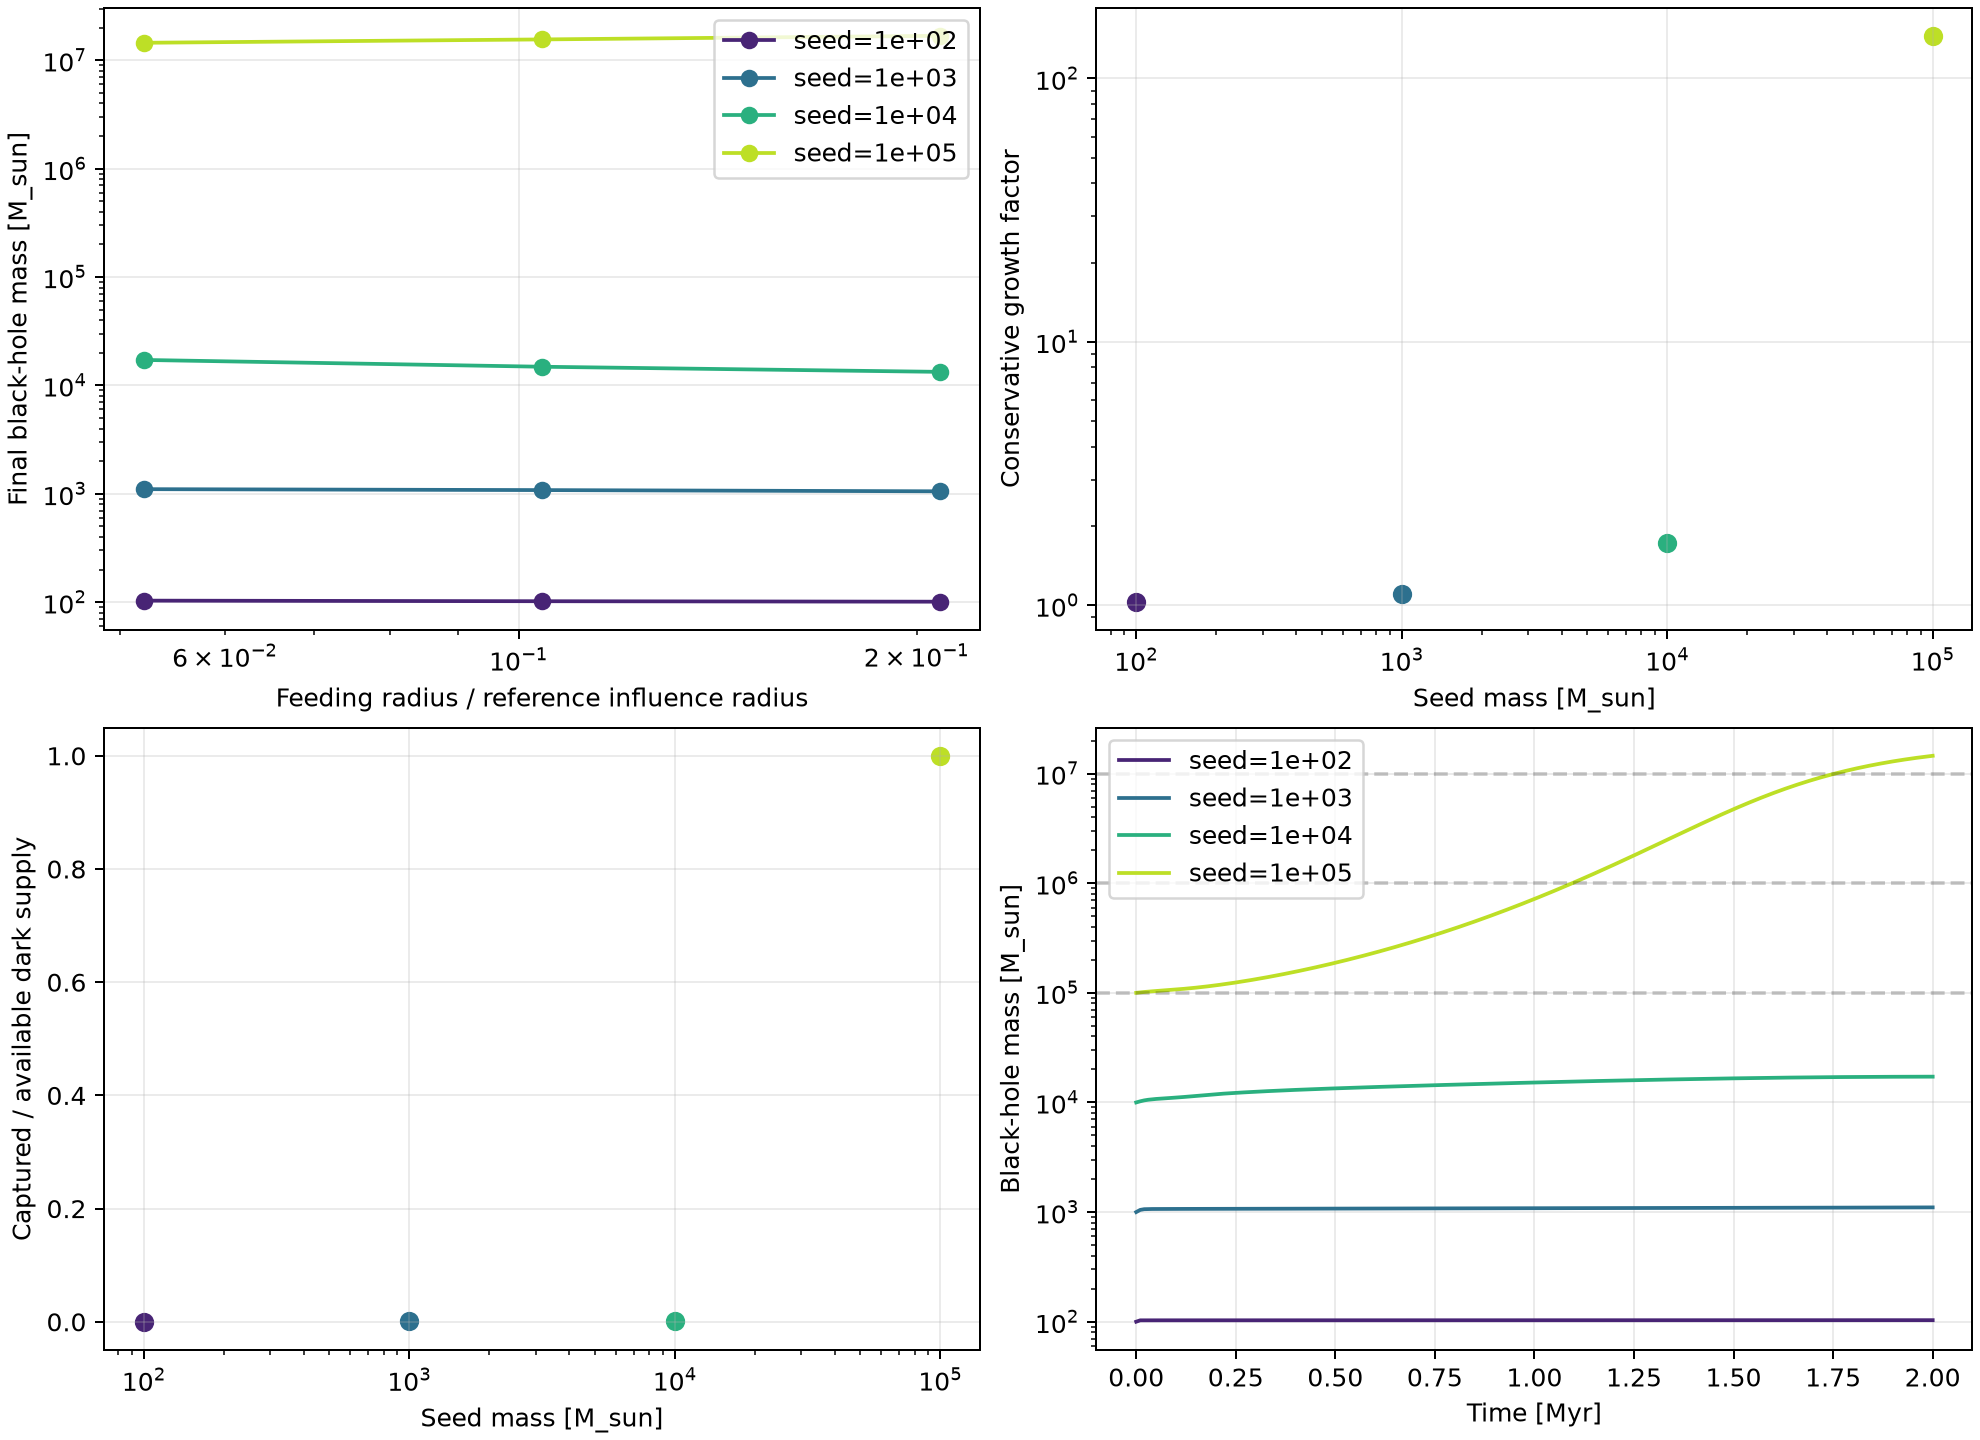
\includegraphics[width=\linewidth]{light_seed_boundary.png}
  \smallskip\centerline{(a) Conservative seed ladder and feeding-boundary prescription.}
 \end{minipage}
 \\
 \begin{minipage}[t]{0.98\linewidth}
  \centering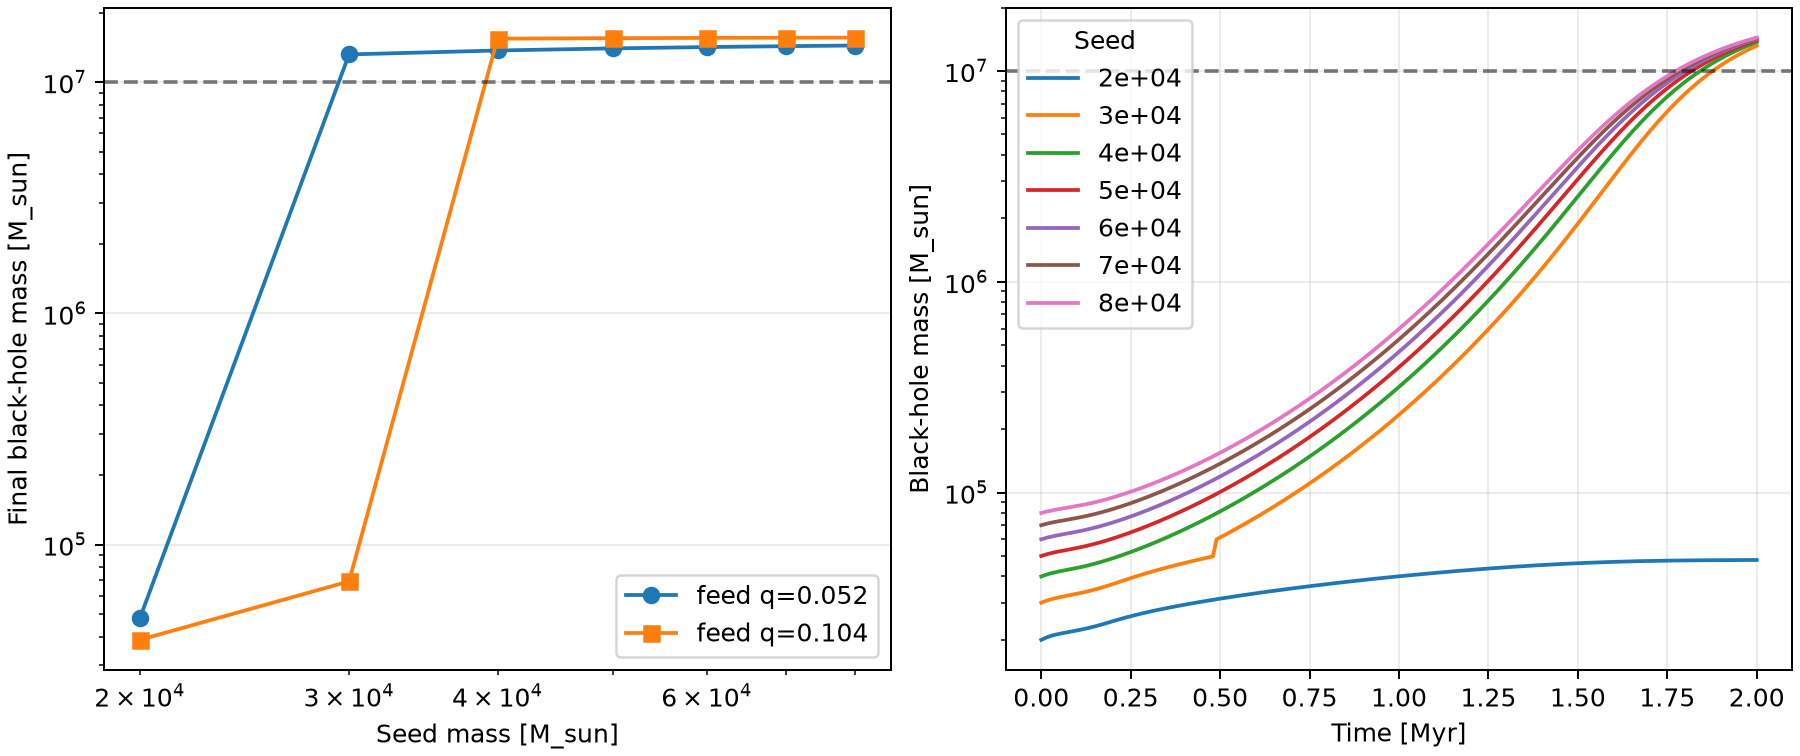
\includegraphics[width=\linewidth]{intermediate_seed_threshold.png}
  \smallskip\centerline{(b) Boundary-bracketed intermediate-seed transition.}
 \end{minipage}
 \caption{Light-seed capture model.  Stellar-remnant seeds remain capture limited even though the SIDM fluid delivers substantial mass to the feeding radius.  The intermediate-seed transition is bracketed rather than uniquely located because it depends on the capture coefficient and feeding boundary.}
 \label{fig:seeds}
\end{figure}

\begin{table}[t]
\centering
\caption{Fixed-halo seed ladder under the fiducial physical-cooling model.}
\label{tab:seeds}
\small
\begin{tabular}{@{}ccccc@{}}
\toprule
$M_{\rm seed}/\msun$ & $M_{\rm BH}(2\,{\rm Myr})/\msun$ & growth & boundary diff. & $10^7\msun$?\\
\midrule
$10^2$ & 103.3 & 1.033 & 1.24\% & no\\
$10^3$ & $1.10\times10^3$ & 1.103 & 1.97\% & no\\
$10^4$ & $1.33$--$1.72\times10^4$ & 1.33--1.72 & 14.4\% & no\\
$10^5$ & $1.452\times10^7$ (conservative) & 145.2 & 7.14\% & yes\\
\bottomrule
\end{tabular}
\end{table}

Refinement over $2\times10^4$--$8\times10^4\msun$ brackets a nonlinear transition.  At nominal $\lambda_B=0.25$, $4\times10^4\msun$ and larger seeds cross $10^7\msun$ at both tested feeding radii, whereas $2\times10^4\msun$ fails.  Seeds between $3\times10^4$ and $3.75\times10^4\msun$ are boundary ambiguous.  Varying $\lambda_B$ from $0.20$ to $0.30$ leaves the $10^2$--$10^4\msun$ failures unchanged at the tested boundaries, but moves the $4\times10^4\msun$ case from failure to a crossing at the single boundary used in that sensitivity pair.

Figure~\ref{fig:capture-map} displays all existing capture-coefficient calculations without interpolation.  The $\lambda_B=0.25$ row distinguishes failures, boundary-ambiguous cases, and crossings at both completed boundaries.  The $\lambda_B=0.20$ and $0.30$ rows contain one boundary per seed and therefore cannot establish a continuous success region.  The map demonstrates that the transition is neither absent nor uniquely located: it is bracketed jointly by seed mass, capture coefficient, and feeding boundary.  The robust result is the failure of $10^2$--$10^4\msun$ seeds throughout the tested $\lambda_B=0.20$--$0.30$ interval; rapid growth from intermediate seeds is conditional on the unresolved capture prescription.

\begin{figure}[t]
 \centering
 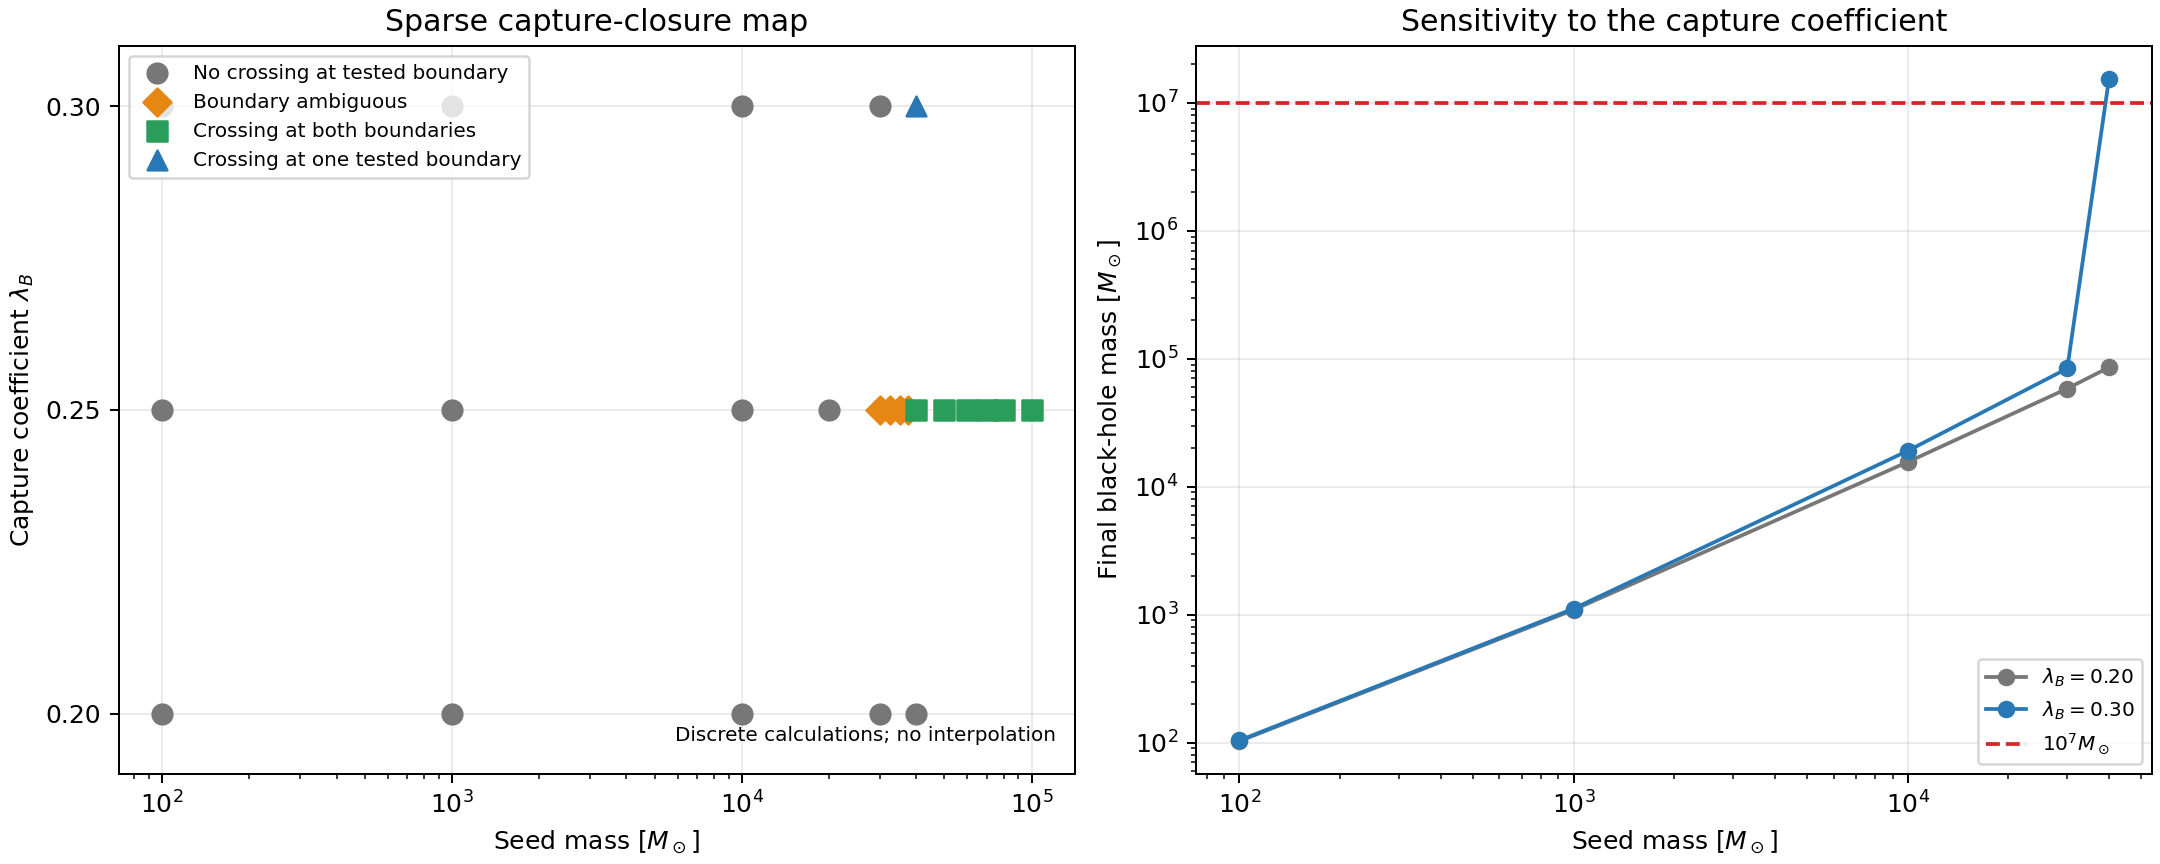
\includegraphics[width=0.98\linewidth]{capture_closure_map.png}
 \caption{Sparse $\lambda_B$--$M_{\rm seed}$ capture map from existing calculations.  Left: discrete threshold classes; triangles denote crossings tested at only one feeding boundary and must not be interpreted as boundary-robust successes.  Right: final masses for the two capture-coefficient sensitivity sequences.  No continuous phase boundary is inferred from these sparse points.}
 \label{fig:capture-map}
\end{figure}

\section{Velocity-dependent cross sections and applicability}
\label{sec:map}

The constant cross section is not the only physically motivated transport law.  We first calibrate the Rutherford transport prescription at the fiducial heavy-seed parameter set.  For $\sigma_0/m=30\,\mathrm{cm^2\,g^{-1}}$, the smaller-boundary endpoints are $1.82\times10^6$, $4.90\times10^6$, and $1.065\times10^7\msun$ for $w=10$, $30$, and $100\kms$, respectively.  The constant control ends at $1.56\times10^7\msun$.  The $w=30\kms$ model has a virial-scale $\sigma_0K_3/m\simeq0.70\,\mathrm{cm^2\,g^{-1}}$, but its initial inner value is only $0.0248\,\mathrm{cm^2\,g^{-1}}$ and it fails the threshold.  Matching the cross section at the virial velocity is therefore not sufficient; the radial and temporal $K_3/K_5$ history matters.

\begin{figure}[t]
 \centering
 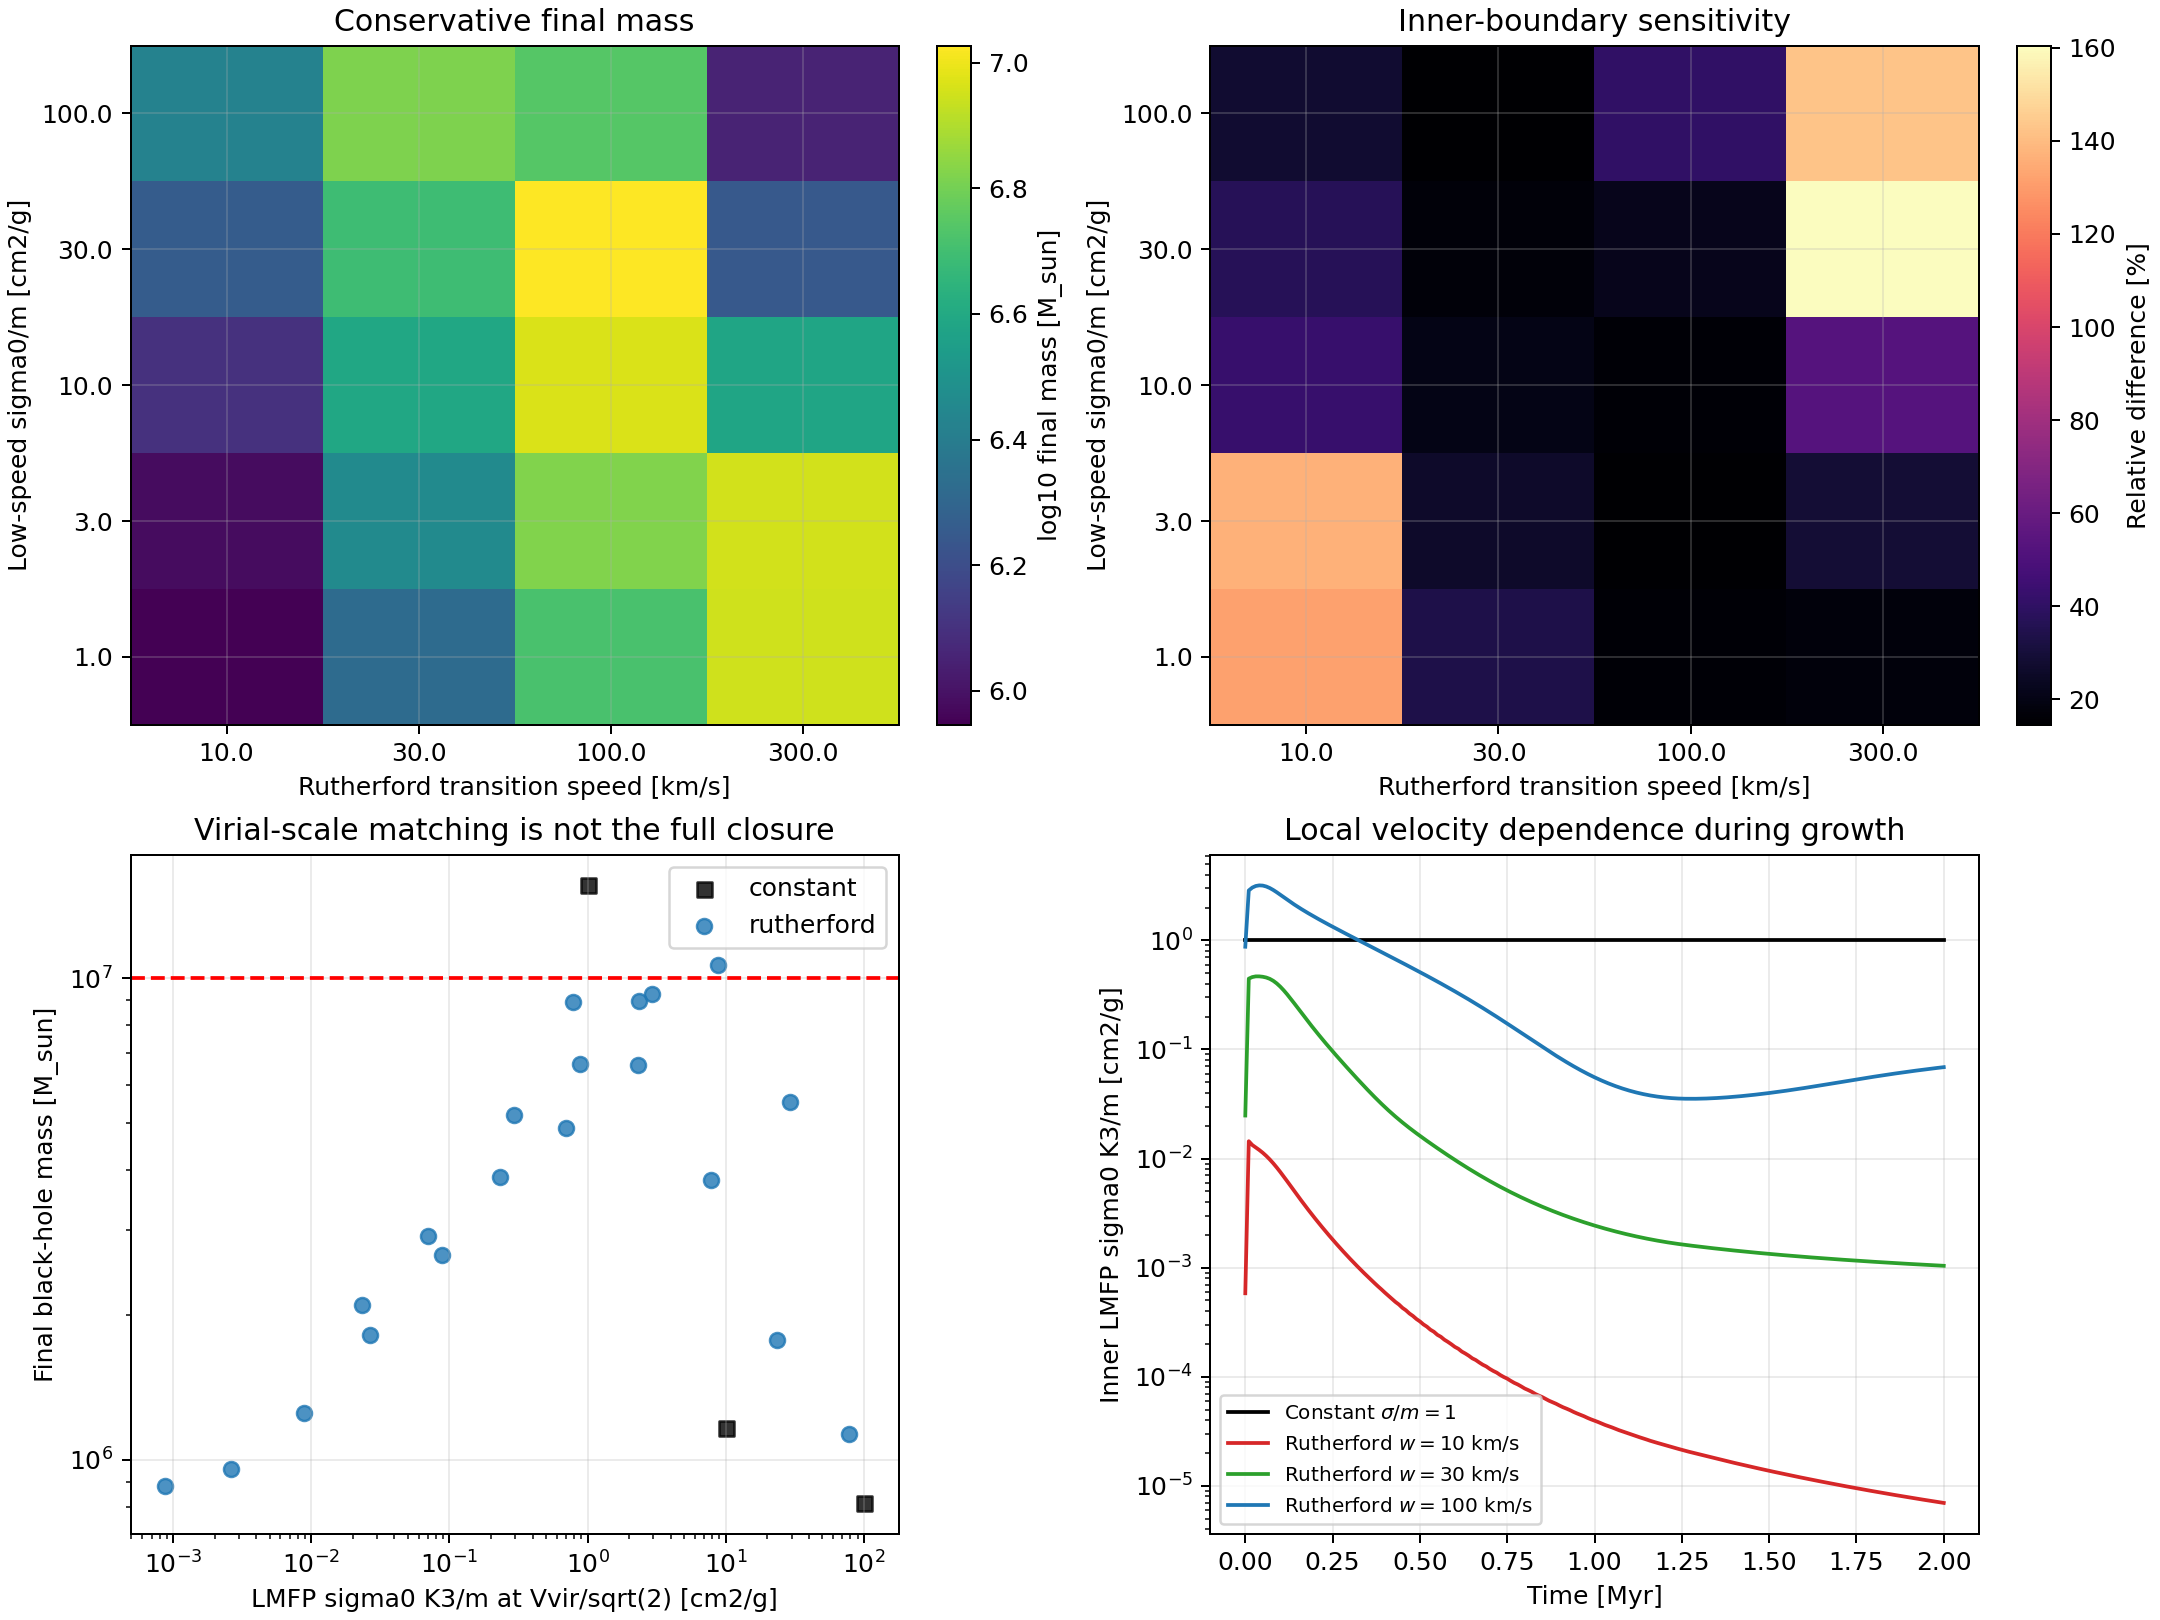
\includegraphics[width=0.98\linewidth]{velocity_transport_calibration.png}
 \caption{Velocity-dependent transport calibration.  The top panels show the conservative final masses and boundary sensitivity as functions of $w$ and $\sigma_0/m$.  The lower panels demonstrate that virial-scale matching does not determine the final mass and that the local effective cross section evolves strongly during growth.}
 \label{fig:velocity}
\end{figure}

We then vary six parameters around the fiducial parameter set: $M_{200}=10^8$--$10^{10}\msun$, $z=15$--$30$, $c=4$--$12$, $M_{\rm seed}=10^2$--$10^5\msun$, $a_b/r_s=0.005$--$0.08$, and $T_{\rm asm}=0.25$--$1.75\,{\rm Myr}$.  Each microphysics model contains 28 one-axis cases and 64 fixed-seed Latin-hypercube cases, followed by boundary and double-grid refinement of the 16 points closest to the threshold.  The initial survey contains 92 points per model; the refined numerical audit contains 16 points per model.  We classify a case as a robust success within the completed numerical bracket only when the threshold crossing survives the smaller-boundary test and, where selected, the double-grid test.  A boundary-ambiguous case crosses in one but not both completed boundaries.  The Latin-hypercube measure is a numerical design, not an astrophysical prior, so sampled fractions are not estimates of cosmic occurrence rates.

\begin{table}[t]
\centering
\caption{Controlled velocity-dependent applicability map.}
\label{tab:map}
\small
\begin{tabular}{@{}lrrrr@{}}
\toprule
model & initial survey & crossings & failures & ambiguous / successes\\
\midrule
constant $\sigma/m=1$ & 92 & 14 & 8 & 2 / 6\\
Rutherford $(\sigma_0,w)=(30,10)$ & 92 & 0 & 16 & 0 / 0\\
Rutherford $(30,30)$ & 92 & 2 & 15 & 1 / 0\\
Rutherford $(30,100)$ & 92 & 16 & 7 & 7 / 2\\
\bottomrule
\end{tabular}
\end{table}

The results are shown in Figure~\ref{fig:map}.  The low-transport $w=10\kms$ model has no threshold crossing anywhere in the initial survey.  The matched $w=30\kms$ model has two initial-survey crossings but no boundary-robust success in its audited neighborhood.  The high-transport $w=100\kms$ model retains two robust points, both in the fiducial halo with $10^5\msun$ seeds and assembly times of $0.5$ or $1.5\,{\rm Myr}$.  The constant control retains six robust audited points, concentrated at high redshift and intermediate-to-heavy seeds.  Across the full refinement no point passes the strict $5\%$ terminal-mass criterion in the combined boundary-plus-grid sense; one low-transport failure happens to pass that numerical metric, which does not alter its threshold class.

Seed mass and redshift show the clearest positive trends in the one-axis and descriptive Latin-hypercube projections, while assembly time and compactness select the width of the crossing window.  These directions are exploratory: the high-transport refinement contains only two boundary-robust successes, both at $M_{\rm seed}=10^5\msun$ in the fiducial halo with $T_{\rm asm}=0.5$ and $1.5\,{\rm Myr}$.  We therefore do not use a sparse logistic fit to assign coefficient significance, success-volume fractions, or population probabilities.

\begin{figure}[t]
 \centering
 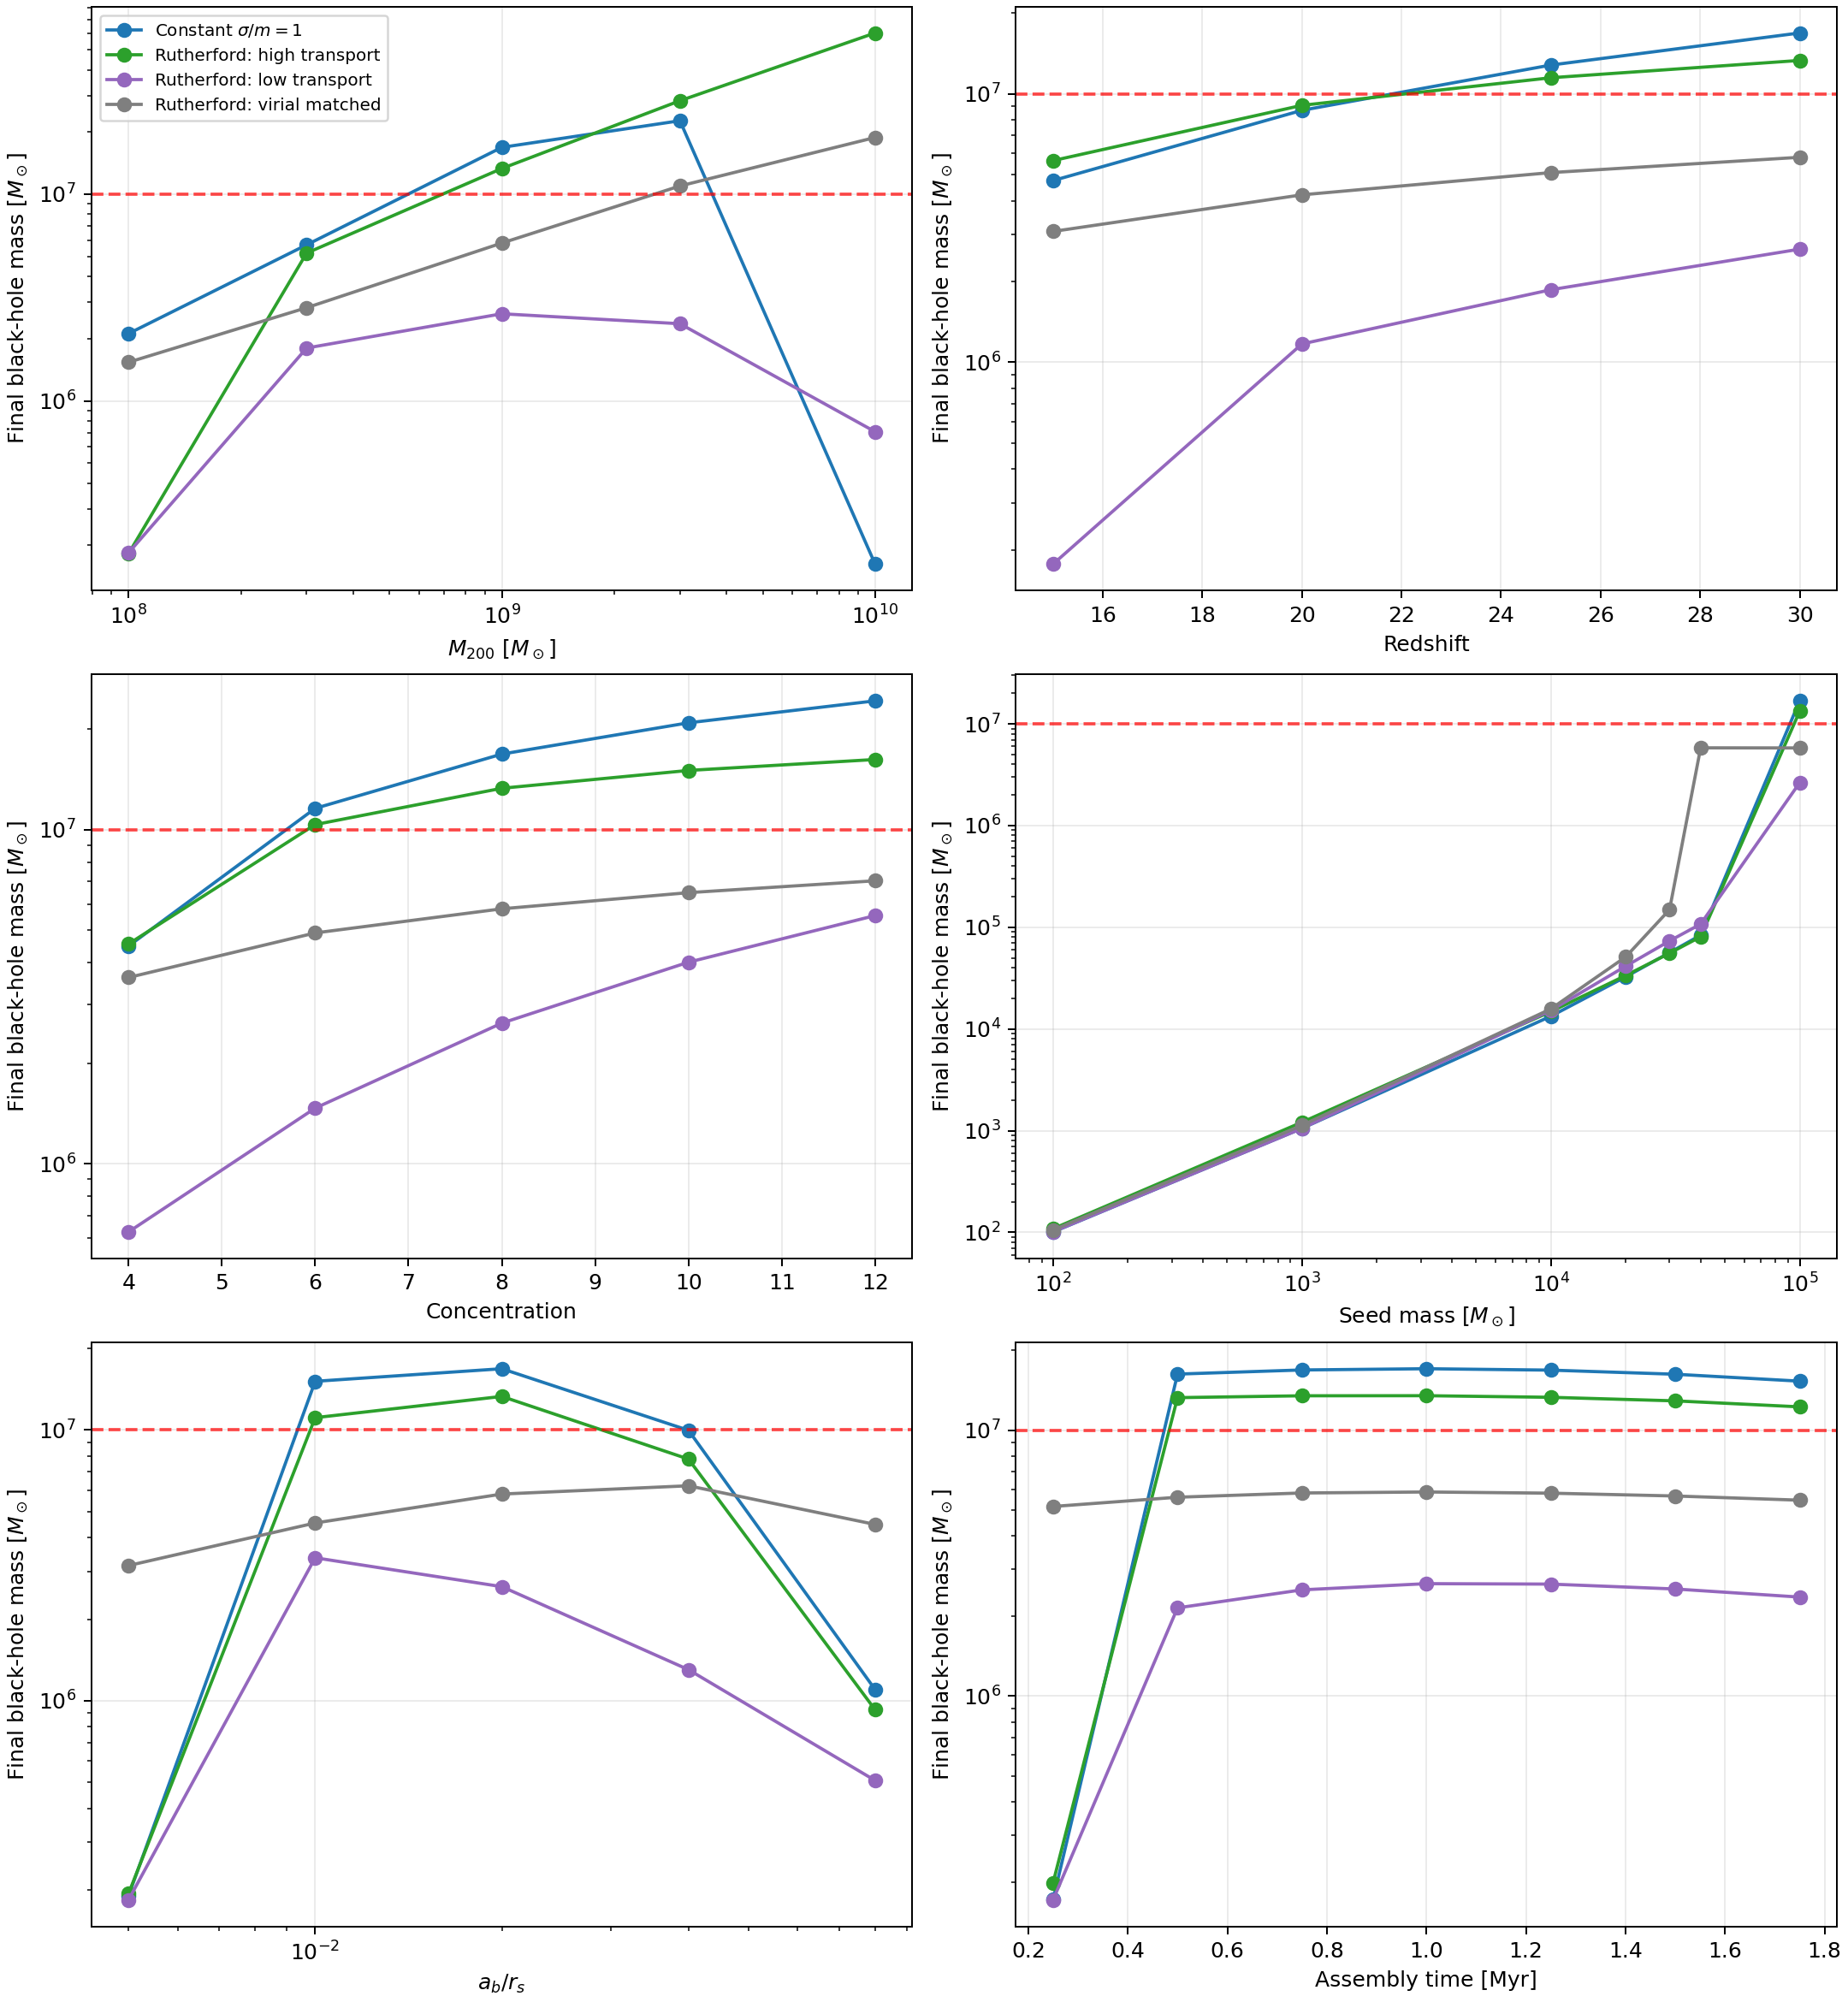
\includegraphics[width=0.98\linewidth]{applicability_main_effects.png}
 \caption{Main effects and joint response in the six-parameter applicability map.  The map is a controlled numerical domain, not a cosmological abundance calculation.}
 \label{fig:map}
\end{figure}

\begin{figure}[t]
 \centering
 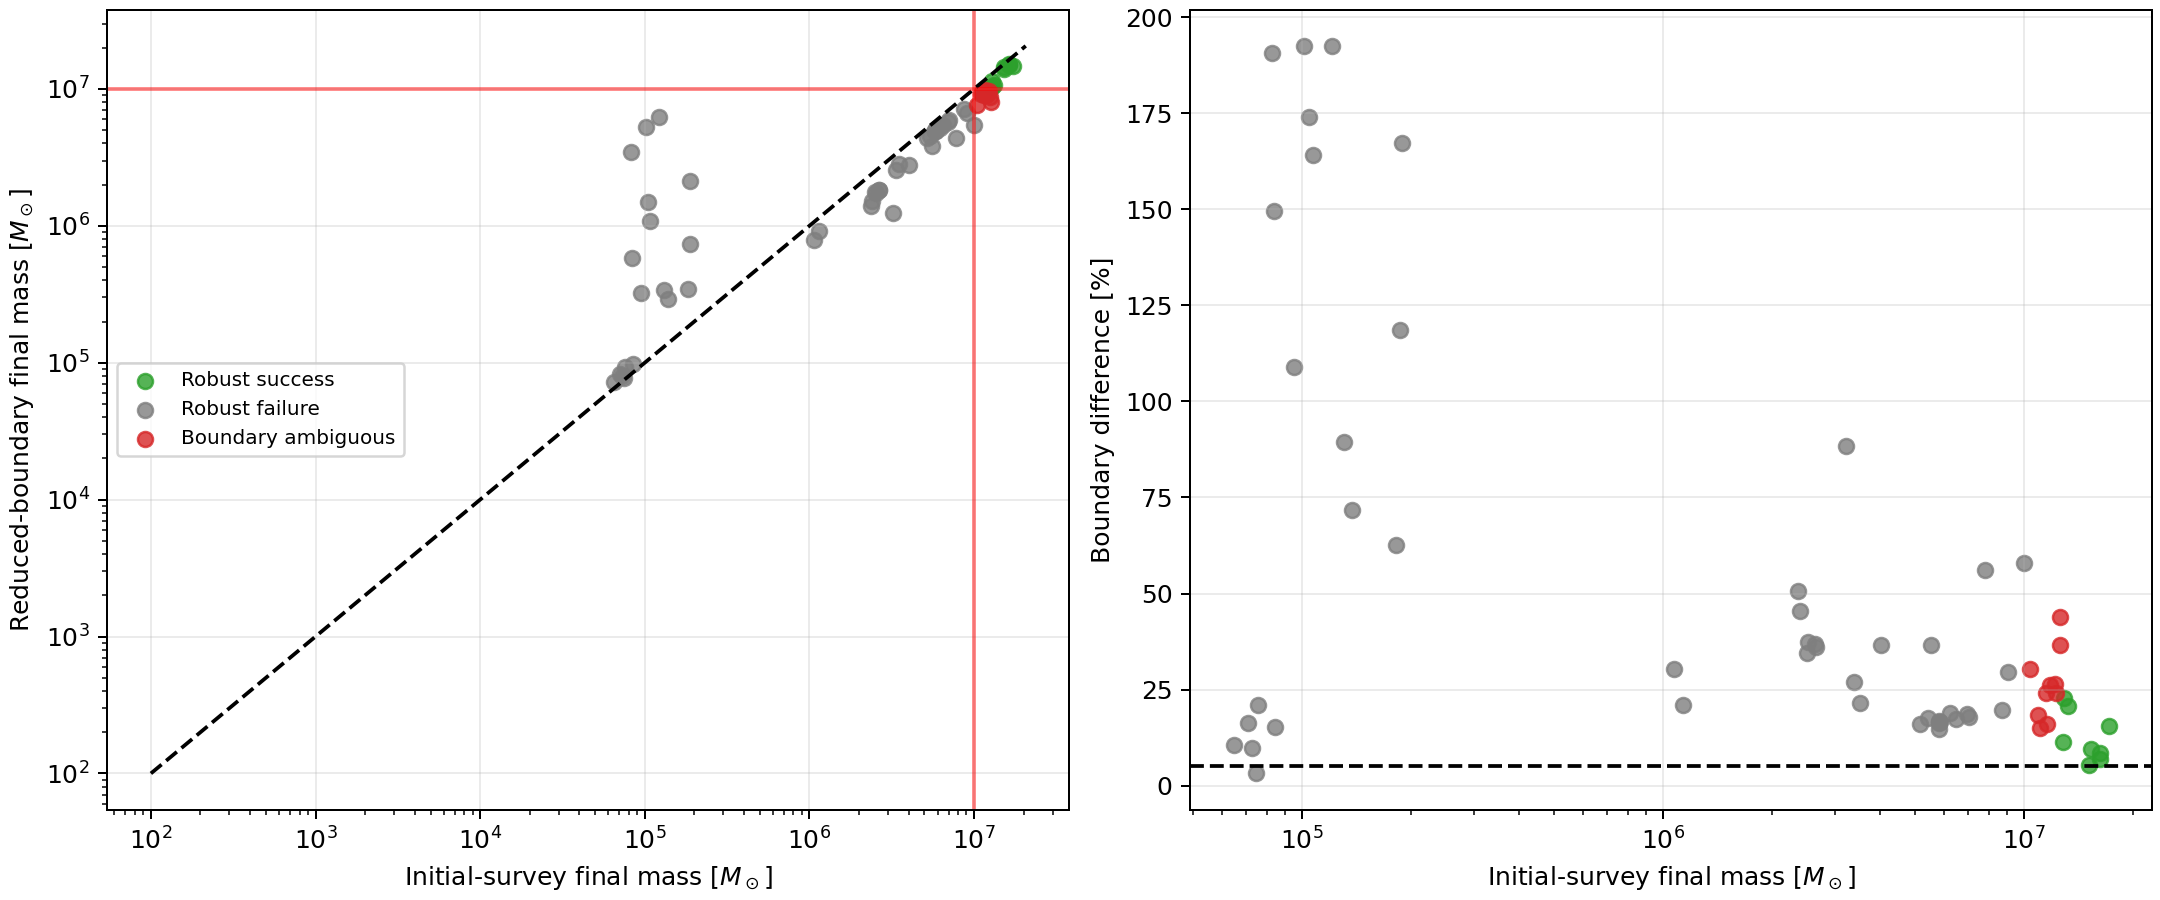
\includegraphics[width=0.98\linewidth]{applicability_boundary_audit.png}
 \caption{Boundary-refined classifications near the $10^7\msun$ threshold.  Threshold crossing is the stable classifier; terminal masses remain provisional when the absorbing inner boundary is unresolved.}
 \label{fig:map-refinement}
\end{figure}

\section{Discussion}
\label{sec:discussion}

\subsection{What is robust}

The first robust conclusion is numerical.  The MC--Roe solver reproduces the reference SIS/NFW histories, and grid, CFL, entropy-fix, and outer-boundary changes are small in comparison with the physical effects.  The remaining dominant numerical systematic is the physical inner boundary.  This distinction matters because the most dramatic nominal endpoints occur precisely where the compact baryonic scale approaches that boundary.

The second robust conclusion is mechanistic.  A growing baryonic potential can enhance SIDM accretion by compressing the supply region, but the response is finite-time and scale dependent.  The preferred assembly time tracks the local dynamical time, while the magnitude of the enhancement is set by conductive heat transport.  The maximum does not occur at the smallest baryonic scale radius.

The third conclusion separates a cooling result from a feedback-model sensitivity.  Under the optically thin table, physical cooling removes stored thermal feedback, so pure heating does not prevent a Bondi-to-Eddington transition unless cooling is suppressed by roughly five orders of magnitude.  Under the adopted irreversible expansion model, mixed expansion can stop the transition by diluting the gas and simultaneously weakens the dark channel.  The sign of this competition is physically interpretable, but the quoted $33\%$ magnitude is model dependent.

The fourth robust conclusion is negative and seed-mass specific.  In the fiducial $10^9\msun$, $z=30$ halo, $10^2$--$10^3\msun$ seeds remain close to their initial masses and $10^4\msun$ seeds remain below $2\times10^4\msun$ throughout the tested capture-coefficient interval.  A $10^5\msun$ seed crosses $10^7\msun$ across the completed boundary bracket.  Between these limits the transition is capture-model and boundary dependent; it is bracketed rather than located as a universal critical mass.

The fifth robust conclusion is restricted to the tested microphysics.  A velocity-dependent cross section can remove every threshold crossing in the sampled domain even when its nominal low-velocity normalization is large.  Only the high-transport $w=100\kms$ model retains boundary-robust examples.  This dependence is controlled by the evolving inner transport averages, not by a single virial velocity.

\subsection{What is not yet a claim}

The calculation is spherically symmetric, has no angular momentum, and uses a one-zone gas environment.  The expansion branch is irreversible and does not include recontraction, multiphase structure, optical-depth effects, or resolved outflows.  The Cloudy table is optically thin and near its high-density limit for the initial ambient state.  The velocity-dependent conductivity is an effective LMFP/SMFP interpolation; anisotropic scattering and merger-driven departures from spherical hydrostatic evolution require independent tests \citep{Robertson2017,Silverman2026}.  Finally, no seed abundance, LRD number density, luminosity function, or spectral observable is inferred here.  Those questions require a population model and are outside the controlled local model presented in this paper.

\section{Conclusions}
\label{sec:conclusions}

We have constructed a matched, time-dependent SIDM--baryon accretion model and followed it from baseline validation to a controlled velocity-dependent applicability map.  The main conclusions are:

\begin{enumerate}
 \item The MC--Roe implementation reproduces the reference SIS/NFW $2\,{\rm Myr}$ endpoints.  Conduction suppresses the final mass by factors of $1.82$ (NFW) and $3.37$ (SIS) relative to the heat-off controls; grid, CFL, entropy-fix, and outer-boundary variations are sub-percent.
 \item An assembled Hernquist potential creates a broad assembly-time window tied to the local dynamical time.  Conductive outward heat transport controls the amplitude, reaching factors of $26.7$--$102.4$ in the refined compact-potential tests.
 \item In the fiducial physical-cooling heavy-seed model, a nominal $1.685\times10^7\msun$ endpoint is not fully boundary converged, but crossing $10^7\msun$ at $1.52$--$1.76\,{\rm Myr}$ survives all completed inner-boundary variants.  The nominal growth is $98.81\%$ dark-matter supplied.  No extrapolation beyond the completed boundary bracket is claimed.
 \item Optically thin cooling erases pure thermal feedback.  Under the adopted irreversible expansion model, mixed feedback can keep the gas Bondi limited and reduce dark accretion by about one third; the magnitude and persistence of this suppression are model sensitivities, not universal predictions.
 \item A conservative feeding-radius prescription separates delivery from capture.  Seeds of $10^2$--$10^4\msun$ do not reach the rapid-growth branch in $2\,{\rm Myr}$ across $\lambda_B=0.20$--$0.30$.  The intermediate-seed transition is bracketed by capture coefficient and feeding boundary rather than identified as a universal critical mass.
 \item Velocity dependence narrows the domain further.  The low-transport Rutherford model has no threshold crossing in the tested six-dimensional domain, whereas the high-transport model retains two boundary-robust heavy-seed examples.  This is a controlled numerical applicability result, not a population-level success fraction.
\end{enumerate}

The next necessary physics extension is a reversible baryon-radius equation with optical-depth and recontraction tests.  A longer integration is useful only after that model ingredient is established; simply extending the present irreversible one-zone model would extrapolate the dominant unresolved systematics rather than add a new robust prediction.

\section*{Acknowledgements}
This work was funded by the National Natural Science Foundation of China (grant No.~11303079) and Zhejiang GuangSha Vocational and Technological University of China (grant No.~2022KYQD-KDB).  The author thanks the maintainers of the Cloudy and Grackle cooling data used in the optically thin treatment and acknowledges computational support from the Paracloud ZC-M6 cluster.

\section*{Data and code availability}
The numerical source, configuration files, machine-readable simulation summaries, convergence logs, and figure-generation scripts are archived at \url{https://github.com/billkang-x/bh-sidm}.  The archived products include the SIS/NFW validation histories, baryonic-assembly scans, cooling and feedback calculations, seed-mass refinements, and the full six-parameter initial survey and numerical follow-up in CSV and JSON formats.  Sampled success fractions are not interpreted as population probabilities.

\bibliographystyle{plainnat}
\bibliography{references}

\end{document}
